%%%%%%%%%%%%%%%%%%%%%%%%%%%%%%%%%%%%%%%%%%%%%%%%%%%%%%%%%%%%%%%%%%%%%%%%
% Beamer Presentation - LaTeX - Template Version 1.0 (10/11/12)
% This template has been downloaded from: http://www.LaTeXTemplates.com
% License: % CC BY-NC-SA 3.0 (http://creativecommons.org/)
% Modified by Rahmat M. Samik-Ibrahim

% REV417: Sun 28 Jan 2024 16:00
% REV398: Wed 02 Nov 2022 13:00
% REV386: Thu 28 Jul 2022 10:00
% REV371: Mon 28 Feb 2022 10:00
% REV363: Mon 20 Dec 2021 15:00
% STARTX: Wed 14 Sep 2016 10:00
%%%%%%%%%%%%%%%%%%%%%%%%%%%%%%%%%%%%%%%%%%%%%%%%%%%%%%%%%%%%%%%%%%%%%%%%%

% PACKAGES AND THEMES 
\documentclass[aspectratio=169, xcolor=table, notheorems, hyperref={pdfpagelabels=false}]{beamer}
%%%%%%%%%%%%%%%%%%%%%%%%%%%%%%%%%%%%%%%%%%%%%%%%%%%%%%%%%%%%%%%%%%%%%%%%
% Beamer Presentation - LaTeX - Template Version 1.0 (10/11/12)
% This template has been downloaded from: http://www.LaTeXTemplates.com
% License: % CC BY-NC-SA 3.0 (http://creativecommons.org/)
% Modified by Rahmat M. Samik-Ibrahim
% REV419: Wed 24 Jul 2024 17:00
% REV383: Tue 12 Jul 2022 10:00
% REV316: Wed 14 Jul 2021 13:00
% REV198: Wed 13 Mar 2019 16:00
% REV005: Mon  2 Oct 2017 14:00
% STARTX: Thu 25 Aug 2016 14:00
%%%%%%%%%%%%%%%%%%%%%%%%%%%%%%%%%%%%%%%%%%%%%%%%%%%%%%%%%%%%%%%%%%%%%%%%%

%% ZCZC NNNN
\newtheorem{example}{Example}

%%%%%%%%%%%%%%%%%%%%%%%%%%%%%%%%%%%%%%%%%%%%%%%%%%%%%%%%%%%%%%%%%%%%%%%%%

\let\Tiny=\tiny
\mode<presentation> {
% The Beamer class comes with a number of default slide themes
% which change the colors and layouts of slides. Below this is a list
% of all the themes, uncomment each in turn to see what they look like.
%\usetheme{Boadilla}
\usetheme{Madrid}
% ZCZC %%%%%%%%%%%%%%%%%%%%%%%%%%%%%%%%%%%%%%%%%%%%%%%%%%%%%%%%%%%%%%%%%%
% \usetheme{default} \usetheme{AnnArbor} \usetheme{Antibes} \usetheme{Bergen}
% \usetheme{Berkeley} \usetheme{Berlin} \usetheme{CambridgeUS} 
% \usetheme{Copenhagen} \usetheme{Darmstadt} \usetheme{Dresden}
% \usetheme{Frankfurt} \usetheme{Goettingen} \usetheme{Hannover}
% \usetheme{Ilmenau} \usetheme{JuanLesPins} \usetheme{Luebeck}
% \usetheme{Malmoe} \usetheme{Marburg} \usetheme{Montpellier}
% \usetheme{PaloAlto} \usetheme{Pittsburgh} \usetheme{Rochester}
% \usetheme{Singapore} \usetheme{Szeged} \usetheme{Warsaw}
% NNNN %%%%%%%%%%%%%%%%%%%%%%%%%%%%%%%%%%%%%%%%%%%%%%%%%%%%%%%%%%%%%%%%%%
% As well as themes, the Beamer class has a number of color themes
% for any slide theme. Uncomment each of these in turn to see how it
% changes the colors of your current slide theme.
%\usecolortheme{orchid}
%\usecolortheme{rose}
%\usecolortheme{seagull}
%\usecolortheme{seahorse}
\usecolortheme{whale}
% ZCZC %%%%%%%%%%%%%%%%%%%%%%%%%%%%%%%%%%%%%%%%%%%%%%%%%%%%%%%%%%%%%%%%%%
%\usecolortheme{albatross} \usecolortheme{beaver} \usecolortheme{beetle}
%\usecolortheme{crane} \usecolortheme{dolphin} \usecolortheme{dove}
%\usecolortheme{fly} \usecolortheme{lily} \usecolortheme{wolverine}
% NNNN %%%%%%%%%%%%%%%%%%%%%%%%%%%%%%%%%%%%%%%%%%%%%%%%%%%%%%%%%%%%%%%%%%
% To remove the footer line in all slides uncomment this line
%\setbeamertemplate{footline} 
% To replace the footer line in all slides uncomment this line
%\setbeamertemplate{footline}[page number] 
% To remove the navigation symbols from the bottom uncomment this line
\setbeamertemplate{navigation symbols}{} 
}

\usepackage{array}       % ZCZC
\usepackage{amssymb}     % ZCZC
\usepackage{bold-extra}  % ZCZC
\usepackage{booktabs}    % Allows \toprule, \midrule and \bottomrule in tables
\usepackage{caption}
\usepackage[T1]{fontenc} % ZCZC << >>
\usepackage{graphicx}    % Allows including images
\usepackage{listings}    % listing
\usepackage{lmodern}     % ZCZC
\usepackage{perpage}     % reset footnote per page
\usepackage{geometry}    % ZCZC
\usepackage{adjustbox}   % ZCZC
\usepackage{multicol}    % ZCZC
\usepackage{multirow}    % ZCZC
\usepackage{pgf-pie}     % ZCZC pie chart

% \definecolor{links}{HTML}{2A1B81}
\definecolor{links}{HTML}{0011FF}
\hypersetup{colorlinks,linkcolor=,urlcolor=links}

% \usepackage{xcolor}
% \usepackage[colorlinks = true,
%             linkcolor = blue,
%             urlcolor  = blue,
%             citecolor = blue,
%             anchorcolor = blue]{hyperref}

\captionsetup[table]{name=Tabel}
\makeatletter
\def\input@path{{src/}}
\makeatother
\graphicspath{{src/}}      % src directory
\MakePerPage{footnote}     % reset page

% NNNN %%%%%%%%%%%%%%%%%%%%%%%%%%%%%%%%%%%%%%%%%%%%%%%%%%%%%%%%%%%%%%%%%%

%% % XXXXXXXXXXXXXXXXXXXXXXXXXXXXXXXXXXXXXXXXXXXXXXXXXXXXXXXXXXXXXXXXXXXXXXXXXX
%% % The short title appears at the bottom of every slide, 
%% % the full title is only on the title page
%% \title[Judul Pendek]{Judul Panjang dan Lengkap} 
%% \author{Cecak bin Kadal}
%% \institute[UILA]
%% {
%% University of Indonesia at Lenteng Agung \\ 
%% \medskip
%% \textit{cecak@binKadal.com}
%% }
%% \date{REV00 24-Aug-2016}
%% % \date{\today}
%% 

%% % XXXXXXXXXXXXXXXXXXXXXXXXXXXXXXXXXXXXXXXXXXXXXXXXXXXXXXXXXXXXXXXXXXXXXXXXXX
%% \begin{document}
%% \section{Judul}
%% \begin{frame}
%% \titlepage
%% \end{frame}
%% 
%% % XXXXXXXXXXXXXXXXXXXXXXXXXXXXXXXXXXXXXXXXXXXXXXXXXXXXXXXXXXXXXXXXXXXXXXXXXX
%% \section{Agenda}
%% \begin{frame}
%% \frametitle{Agenda}
%% % Throughout your presentation, if you choose to use \section{} and 
%% % \subsection{} commands, these will automatically be printed on 
%% % this slide as an overview of your presentation
%% \tableofcontents 
%% \end{frame}
%% 
%% % XXXXXXXXXXXXXXXXXXXXXXXXXXXXXXXXXXXXXXXXXXXXXXXXXXXXXXXXXXXXXXXXXXXXXXXXXX
%% \section{UUD dan Pancasila}
%% \subsection{UUD}
%% \begin{frame}
%% \frametitle{Pembukaan}
%% Bahwa sesungguhnya kemerdekaan itu ialah hak segala bangsa dan oleh 
%% sebab itu, maka penjajahan diatas dunia harus dihapuskan karena 
%% tidak sesuai dengan perikemanusiaan dan perikeadilan.
%% \\~\\
%% Atas berkat rahmat Allah Yang Maha Kuasa dan dengan didorongkan oleh 
%% keinginan luhur, supaya berkehidupan kebangsaan yang bebas, maka 
%% rakyat Indonesia menyatakan dengan ini kemerdekaannya.
%% \end{frame}
%% 
%% % XXXXXXXXXXXXXXXXXXXXXXXXXXXXXXXXXXXXXXXXXXXXXXXXXXXXXXXXXXXXXXXXXXXXXXXXXX
%% \begin{frame}
%% \frametitle{Alenia Ketiga}
%% Kemudian daripada itu untuk membentuk suatu pemerintah negara Indonesia 
%% yang melindungi segenap bangsa Indonesia dan seluruh tumpah darah Indonesia 
%% dan untuk memajukan kesejahteraan umum, mencerdaskan kehidupan bangsa, dan 
%% ikut melaksanakan ketertiban dunia yang berdasarkan kemerdekaan, perdamaian 
%% abadi dan keadilan sosial, maka disusunlah kemerdekaan kebangsaan Indonesia 
%% itu dalam suatu Undang-Undang Dasar negara Indonesia, yang terbentuk dalam 
%% suatu susunan negara Republik Indonesia yang berkedaulatan rakyat dengan 
%% berdasar kepada:
%% \begin{itemize}
%% \item Ketuhanan Yang Maha Esa,
%% \item kemanusiaan yang adil dan beradab,
%% \item persatuan Indonesia,
%% \item dan kerakyatan yang dipimpin oleh hikmat kebijaksanaan 
%%       dalam permusyawaratan/ perwakilan,
%% \item serta dengan mewujudkan suatu keadilan sosial bagi seluruh rakyat 
%%       Indonesia.
%% \end{itemize}
%% \end{frame}
%% 
%% % XXXXXXXXXXXXXXXXXXXXXXXXXXXXXXXXXXXXXXXXXXXXXXXXXXXXXXXXXXXXXXXXXXXXXXXXXX
%% \subsection{Pancasila}
%% \begin{frame}
%% \frametitle{Tujuh Kunci Pokok}
%% \begin{block}{Pertama - Kedua - Ketiga}
%% Indonesia ialah negara berdasarkan hukum.
%% Sistem konstitusional.
%% Kekuasaan negara tertinggi di tangan MPR.
%% \end{block}
%% 
%% \begin{block}{Keempat - Kelima}
%% Presiden adalah penyelenggara pemerintahan tertinggi di bawah MPR.
%% Adanya pengawasan DPR.
%% \end{block}
%% 
%% \begin{block}{Keenam}
%% Menteri negara adalah pembantu presiden dan tidak bertanggung jawab 
%% kepada DPR.
%% \end{block}
%% 
%% \begin{block}{Ketujuh}
%% Kekuasaan kepala negara tidak tak tebatas.
%% \end{block}
%% 
%% \end{frame}
%% 
%% % XXXXXXXXXXXXXXXXXXXXXXXXXXXXXXXXXXXXXXXXXXXXXXXXXXXXXXXXXXXXXXXXXXXXXXXXXX
%% \section{Rupa-rupa}
%% \subsection{Kolom}
%% \begin{frame}
%% \frametitle{Kolom}
%% % The "c" option specifies centered vertical alignment 
%% % while the "t" option is used for top vertical alignment
%% \begin{columns}[c] 
%% % Left column and width
%% \column{.45\textwidth} 
%% \textbf{Heading}
%% \begin{enumerate}
%% \item Satu-satu
%% \item Dua-dua
%% \item Tiga-tiga
%% \item Satu-dua-tiga
%% \end{enumerate}
%% 
%% % Right column and width
%% \column{.5\textwidth}
%% Satu-satu~\dots{} aku sayang ibu!
%% Dua-dua~\ldots{} juga sayang ayah!
%% Tiga-tiga~\ldots{} sayang adik kakak!
%% Satu-dua-tiga~\ldots{} sayang semuanya!
%% 
%% \end{columns}
%% \end{frame}
%% 
%% % XXXXXXXXXXXXXXXXXXXXXXXXXXXXXXXXXXXXXXXXXXXXXXXXXXXXXXXXXXXXXXXXXXXXXXXXXX
%% \subsection{Tabel}
%% \begin{frame}
%% \frametitle{Tabel}
%% \begin{table}
%% \begin{tabular}{l l l}
%% \toprule
%% \textbf{Nama} & \textbf{NPM} & \textbf{Tanggal Lahir}\\
%% \midrule
%% Cecak bin Kadal & 1234567890 & 1 Jan 2015 \\
%% Aneh bin Ajaib  & 0987654321 & 31 Des 2014 \\
%% \bottomrule
%% \end{tabular}
%% \caption{Keterangan Tabel}
%% \end{table}
%% \end{frame}
%% 
%% % XXXXXXXXXXXXXXXXXXXXXXXXXXXXXXXXXXXXXXXXXXXXXXXXXXXXXXXXXXXXXXXXXXXXXXXXXX
%% \subsection{Teori}
%% \begin{frame}
%% \frametitle{Teori}
%% \begin{theorem}[Teori Satu Batu]
%% $E = mc^2$
%% \end{theorem}
%% \end{frame}
%% 
%% % XXXXXXXXXXXXXXXXXXXXXXXXXXXXXXXXXXXXXXXXXXXXXXXXXXXXXXXXXXXXXXXXXXXXXXXXXX
%% \subsection{Verbatim}
%% % Need to use the fragile option when verbatim is used in the slide
%% \begin{frame}[fragile] 
%% \frametitle{Verbatim}
%% \begin{example}[Teori Satu Batu]
%% \begin{verbatim}
%% \begin{theorem}[Teori Satu Batu]
%% $E = mc^2$
%% \end{theorem}
%% \end{verbatim}
%% \end{example}
%% \end{frame}
%% 
%% % XXXXXXXXXXXXXXXXXXXXXXXXXXXXXXXXXXXXXXXXXXXXXXXXXXXXXXXXXXXXXXXXXXXXXXXXXX
%% \subsection{Gambar}
%% \begin{frame}
%% \frametitle{Gambar}
%% \begin{figure}
%% \includegraphics[width=0.5\linewidth]{2}
%% \caption{Ini Gambar JPG}
%% \end{figure}
%% \end{frame}
%% 
%% % XXXXXXXXXXXXXXXXXXXXXXXXXXXXXXXXXXXXXXXXXXXXXXXXXXXXXXXXXXXXXXXXXXXXXXXXXX
%% \subsection{Rujukan}
%% % Need to use the fragile option when verbatim is used in the slide
%% \begin{frame}[fragile] 
%% \frametitle{Rujukan dan Kutipan}
%% Contoh penggunaan \verb|\cite| ketika mengutip\cite{p1}.
%% Perhatian: Beamer tidak mengerti \verb|\BibTeX|~\ldots
%% \footnotesize{
%%   \begin{thebibliography}{99} 
%%   \bibitem[Smith, 2012]{p1} John Smith (2012)
%%      \newblock Katak dalam Tempurung
%%      \newblock \emph{Jurnal Kelapa dan Amfibi} 12(3), 45 -- 678.
%%   \end{thebibliography}
%% }
%% \end{frame}
%% 
%% % XXXXXXXXXXXXXXXXXXXXXXXXXXXXXXXXXXXXXXXXXXXXXXXXXXXXXXXXXXXXXXXXXXXXXXXXXX
%% \subsection{Selesai}
%% \begin{frame}
%% \Huge{\centerline{Selesai}}
%% \end{frame}
%% 
%% % XXXXXXXXXXXXXXXXXXXXXXXXXXXXXXXXXXXXXXXXXXXXXXXXXXXXXXXXXXXXXXXXXXXXXXXXXX
%% \end{document}

\newcommand{\revision}{%
REV426: Wed 13 Nov 2024 04:00
}
% w! tmptmp
% REV426: Wed 13 Nov 2024 04:00
% REV419: Wed 24 Jul 2024 17:00
% REV409: Tue 08 Aug 2023 12:00
% REV399: Fri 03 Feb 2023 20:00
% REV339: Sat 04 Sep 2021 12:00
% STARTS: Wed 24 Aug 2016 19:00
%%%%%%%%%%%%%%%%%%%%%%%%%%%%%%%%%%%%%
\newcommand{\kopikopi}{\textcopyright{}2016-2024 CBKadal + VauLSMorg}



% XXXXXXXXXXXXXXXXXXXXXXXXXXXXXXXXXXXXXXXXXXXXXXXXXXXXXXXXXXXXXXXXXXXXXXXXXX
% The short title appears at the bottom of every slide, 
% the full title is only on the title page
% \date{\today}
\title[\kopikopi]
{CSGE602055 Operating Systems \\ 
CSF2600505 Sistem Operasi \\
Week 06:
Concurrency: Processes \& Threads}
\author{C. BinKadal}
\institute[SdnBhd]
{
Sendirian Berhad\\
\medskip
\url{https://docOS.vlsm.org/Slides/os06.pdf}
\\ \texttt{Always check for the latest revision!}
}
\date{\revision}

% XXXXXXXXXXXXXXXXXXXXXXXXXXXXXXXXXXXXXXXXXXXXXXXXXXXXXXXXXXXXXXXXXXXXXXXXXX
\begin{document}

\lstset{
basicstyle=\ttfamily\tiny, % \tiny \small \footnotesize 
breakatwhitespace=true,
language=C,
columns=fullflexible,
keepspaces=true,
breaklines=true,
tabsize=3, 
showstringspaces=false,
extendedchars=true}

\section{Start}
\begin{frame}
\titlepage
\end{frame}

% XXXXXXXXXXXXXXXXXXXXXXXXXXXXXXXXXXXXXXXXXXXXXXXXXXXXXXXXXXXXXXXXXXXXXXXXXX

%%%%%%%%%%%%%%%%%%%%%%%%%%%%%%%%%%%%%%%%%%%%%%%%%%%%%%%%%%%%%%%%%%%%%%%%%
% REV418: Tue 30 Jan 2024 22:00
% REV406: Sat 05 Aug 2023 14:00
% REV399: Thu 02 Feb 2023 00:00
% REV369: Mon 14 Feb 2022 09:00
% REV328: Sat 14 Aug 2021 06:00
% STARTX: Wed 14 Sep 2016 10:00
%%%%%%%%%%%%%%%%%%%%%%%%%%%%%%%%%%%%%%%%%%%%%%%%%%%%%%%%%%%%%%%%%%%%%%%%%

\begin{frame}[fragile]
\section{OS241 Schedule}
\frametitle{OS241\footnote{%
) This information will be on \textbf{EVERY} page two (2) of this course material.}): 
Operating Systems Schedule 2023 - 2}

\vspace{5pt}

\scalebox{0.99}{%
\begin{tabular}{|c|c|l|l|}
\hline
\textbf{Week} & 
\textbf{Topic}\footnote{%
) For schedule, see \url{https://os.vlsm.org/\#idx02}}) & \textbf{OSC10}\footnote{%
    ) Silberschatz et. al.: \textbf{Operating System Concepts}, $10^{th}$ Edition, 2018.}) \\
\hline
Week 00  & Overview (1), Assignment of Week 00           & Ch. 1, 2      \\
Week 01  & Overview (2), Virtualization \& Scripting     & Ch. 1, 2, 18. \\
Week 02  & Security, Protection, Privacy, \& C-language. & Ch. 16, 17.   \\
Week 03  & File System \& FUSE  & Ch. 13, 14, 15.                        \\
Week 04  & Addressing, Shared Lib, \& Pointer & Ch. 9. \\
Week 05  & Virtual Memory & Ch. 10. \\
\hline
Week 06  & Concurrency: Processes \& Threads & Ch. 3, 4. \\
Week 07  & Synchronization \& Deadlock & Ch. 6, 7, 8. \\
Week 08  & Scheduling + W06/W07 & Ch. 5. \\
Week 09  & Storage, Firmware, Bootloader, \& Systemd & Ch. 11. \\
Week 10  & I/O \& Programming & Ch. 12. \\%
% MidTerm  & 00 XXX 2020 (XX:XX-XX:XX) & MidTerm (UTS) & \cellcolor{red!44} TBA! \\
% Reserved & 00 XXX - 00 XXX 2020 & Q \& A & \\
% Final    & 00 XXX 2020 XX:XX & First Part Final  (UAS tahap I)  & \cellcolor{red!44} This schedule is   \\
% Extra    & NA & No Extra assignment & \cellcolor{red!44} subject to change. \\
\hline
\end{tabular}
}
\end{frame}

\begin{frame}[fragile]
\frametitle{\textbf{STARTING POINT} --- 
{
\definecolor{links}{HTML}{FDEE00}
\hypersetup{colorlinks,linkcolor=,urlcolor=links}
\url{https://os.vlsm.org/}
}
}
\begin{itemize}
\item[$\square$] \textbf{Text Book} ---
                 Any recent/decent OS book. Eg. (\textbf{OSC10}) Silberschatz et. al.: 
                 \textbf{Operating System Concepts}, $10^{th}$ Edition, 2018.
                 (See \url{https://codex.cs.yale.edu/avi/os-book/OS10/}).
\item[$\square$] \textbf{Resources ({\footnotesize \url{https://os.vlsm.org/\#idx03}})}
\begin{itemize}
\item[$\square$] \href{https://scele.cs.ui.ac.id/course/view.php?id=3743}{\textbf{SCELE}} ---
\url{https://scele.cs.ui.ac.id/course/view.php?id=3743}.\\
The enrollment key is \textbf{XXX}.
\item[$\square$] \textbf{Download Slides and Demos from GitHub.com} --- (\url{https://github.com/os2xx/docOS/})\\
                 {\scriptsize%
                 \href{https://docOS.vlsm.org/Slides/os00.pdf}{\texttt{os00.pdf} (W00)},
                 \href{https://docOS.vlsm.org/Slides/os01.pdf}{\texttt{os01.pdf} (W01)},
                 \href{https://docOS.vlsm.org/Slides/os02.pdf}{\texttt{os02.pdf} (W02)},
                 \href{https://docOS.vlsm.org/Slides/os03.pdf}{\texttt{os03.pdf} (W03)},
                 \href{https://docOS.vlsm.org/Slides/os04.pdf}{\texttt{os04.pdf} (W04)},
                 \href{https://docOS.vlsm.org/Slides/os05.pdf}{\texttt{os05.pdf} (W05)},\\
                 \href{https://docOS.vlsm.org/Slides/os06.pdf}{\texttt{os06.pdf} (W06)},
                 \href{https://docOS.vlsm.org/Slides/os07.pdf}{\texttt{os07.pdf} (W07)},
                 \href{https://docOS.vlsm.org/Slides/os08.pdf}{\texttt{os08.pdf} (W08)},
                 \href{https://docOS.vlsm.org/Slides/os09.pdf}{\texttt{os09.pdf} (W09)},
                 \href{https://docOS.vlsm.org/Slides/os10.pdf}{\texttt{os10.pdf} (W10)}.
                 }
\item[$\square$] \textbf{Problems}\\
                 {\scriptsize% 
                 \href{https://rms46.vlsm.org/2/195.pdf}{\texttt{195.pdf} (W00)},
                 \href{https://rms46.vlsm.org/2/196.pdf}{\texttt{196.pdf} (W01)},
                 \href{https://rms46.vlsm.org/2/197.pdf}{\texttt{197.pdf} (W02)},
                 \href{https://rms46.vlsm.org/2/198.pdf}{\texttt{198.pdf} (W03)},
                 \href{https://rms46.vlsm.org/2/199.pdf}{\texttt{199.pdf} (W04)},
                 \href{https://rms46.vlsm.org/2/200.pdf}{\texttt{200.pdf} (W05)},\\
                 \href{https://rms46.vlsm.org/2/201.pdf}{\texttt{201.pdf} (W06)},
                 \href{https://rms46.vlsm.org/2/202.pdf}{\texttt{202.pdf} (W07)},
                 \href{https://rms46.vlsm.org/2/203.pdf}{\texttt{203.pdf} (W08)},
                 \href{https://rms46.vlsm.org/2/204.pdf}{\texttt{204.pdf} (W09)},
                 \href{https://rms46.vlsm.org/2/205.pdf}{\texttt{205.pdf} (W10)}.}
\item[$\square$] \textbf{LFS} --- \url{http://www.linuxfromscratch.org/lfs/view/stable/}
\item[$\square$] \textbf{OSP4DISS} --- \url{https://osp4diss.vlsm.org/}
\item[$\square$] \textbf{This is How Me Do It!} --- \url{https://doit.vlsm.org/}
\begin{itemize}
\item[$\square$] PS: "Me" rhymes better than "I", duh!
\end{itemize}
\end{itemize}
\end{itemize}
\end{frame}



% XXXXXXXXXXXXXXXXXXXXXXXXXXXXXXXXXXXXXXXXXXXXXXXXXXXXXXXXXXXXXXXXXXXXXXXXXX
% Throughout your presentation, if you choose to use \section{} and 
% \subsection{} commands, these will automatically be printed on 
% this slide as an overview of your presentation
\section{Agenda}
\begin{frame}{Outline}
  \frametitle{Agenda}
  \tableofcontents[sections={1-15}]
\end{frame}
\begin{frame}
   \frametitle{Agenda (2)}
   \tableofcontents[sections={16-}]
\end{frame}

% XXXXXXXXXXXXXXXXXXXXXXXXXXXXXXXXXXXXXXXXXXXXXXXXXXXXXXXXXXXXXXXXXXXXXXXXXX

%%%%%%%%%%%%%%%%%%%%%%%%%%%%%%%
% REV412: Tue 22 Aug 2023 14:00
% REV406: Sat 05 Aug 2023 12:00
% REV211: Fri 01 Nov 2019 01:00
% REV154: Thu 23 Aug 2018 11:00
% START0: Thu 26 Jul 2018 20:00
%%%%%%%%%%%%%%%%%%%%%%%%%%%%%%%

\section{Week 06}
\begin{frame}[fragile]
\frametitle{Week 06 Concurrency:
Topics\footnote{Source: ACM IEEE CS Curricula}}

\begin{itemize}
\item States and state diagrams 
\item Structures (ready list, process control blocks, and so forth) 
\item Dispatching and context switching 
\item The role of interrupts 
\item Managing atomic access to OS objects 
\item Implementing synchronization primitives 
\item Multiprocessor issues (spin-locks, reentrancy)  
\end{itemize}
\end{frame}

\begin{frame}[fragile]
\frametitle{Week 06 Concurrency:
Learning Outcomes (1)\footnote{Source: ACM IEEE CS Curricula}}
\begin{itemize}
\item Describe the need for concurrency within the framework of an operating system. [Familiarity] 
\item Demonstrate the potential run-time problems arising from the concurrent operation of many separate tasks. [Usage] 
\item Summarize the range of mechanisms that can be employed at the operating system level to realize concurrent systems and describe the benefits of each. [Familiarity] 
\item Explain the different states that a task may pass through and the data structures needed to support the management of many tasks. [Familiarity] 
\end{itemize}
\end{frame}


\begin{frame}[fragile]
\frametitle{Week 06 Concurrency:
Learning Outcomes (2)\footnote{Source: ACM IEEE CS Curricula 2023 (beta)}}
\begin{itemize}
\item Summarize techniques for achieving synchronization in an operating system (e.g., describe how to implement a semaphore using OS primitives). [Familiarity] 
\item Describe reasons for using interrupts, dispatching, and context switching to support concurrency in an operating system. [Familiarity] 
\item Create state and transition diagrams for simple problem domains. [Usage] 
\end{itemize}
\end{frame}



% XXXXXXXXXXXXXXXXXXXXXXXXXXXXXXXXXXXXXXXXXXXXXXXXXXXXXXXXXXXXXXXXXXXXXXXXXX
\section{OSC10 (Silberschatz) Chapter 3: Processes and Chapter 4: Threads \& Concurrency}

\begin{frame}
\frametitle{OSC10 (Silberschatz) Chapter 3 and Chapter 4}
\begin{multicols}{2}
  \begin{itemize}
  \item Chapter 3: Processes 
  \begin{itemize}
  \item Process Concept
  \item Process Scheduling
  \item Operations on Processes
  \item Interprocess Communication
  \item IPC in Shared-Memory Systems
  \item IPC in Message-Passing Systems
  \item Examples of IPC Systems
  \item Communication in Client-Server Systems
  \end{itemize}
  \end{itemize}
  \vfill \null
\columnbreak
  \begin{itemize}
  \item Chapter 4: Threads \& Concurrency
  \begin{itemize}
  \item Overview
  \item Multicore Programming
  \item Multithreading Models
  \item Thread Libraries
  \item Implicit Threading
  \item Threading Issues
  \item Operating System Examples
  \end{itemize}
  \end{itemize}
  \vfill \null
\end{multicols}
\end{frame}

% XXXXXXXXXXXXXXXXXXXXXXXXXXXXXXXXXXXXXXXXXXXXXXXXXXXXXXXXXXXXXXXXXXXXXXXXXX
\section{Week 06}
\begin{frame}[fragile]
\frametitle{Week 06: Concurrency: Processes \& Threads}
\begin{itemize}
\item Reference: (OSC10-ch03 OSC10-ch04 demo-w06)
\item Process Concept
\begin{itemize}
\item Program (passive) $\leftrightarrow$ Process (active)
\item Process in Memory: $ \mid Stack \cdots Heap \mid Data \mid Text \mid $
\item Process State: $ \mid running \mid waiting \mid ready \mid $
\item Process Control Block (PCB)
\begin{itemize}
\item \texttt{/proc/}, Process State, Program Counter, Registers, Management Information.
\end{itemize}
\end{itemize}
\item Process Creation
\begin{itemize}
\item PID: Process Identifier (uniq)
\item The Parent Process forms a tree of Children Processes
\item \texttt{fork()}, new process system call (clone)
\item \texttt{execlp()}, replaces the clone with a new program.
\end{itemize}
\item Process Termination
\begin{itemize}
\item \texttt{wait()}, until the child process is terminated.
\end{itemize}
\item PCB (Context) Switch
\end{itemize}
\end{frame}

% XXXXXXXXXXXXXXXXXXXXXXXXXXXXXXXXXXXXXXXXXXXXXXXXXXXXXXXXXXXXXXXXXXXXXXXXXX
\section{Process Map}
\begin{frame}[fragile]
\frametitle{Process Map (1)}
\begin{figure}
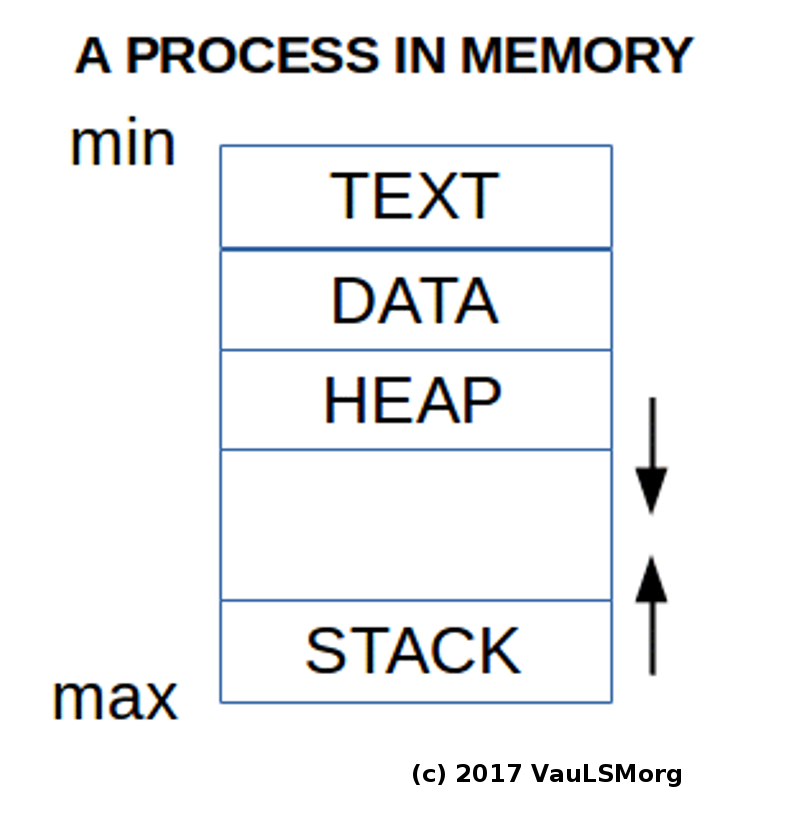
\includegraphics[width=0.43\linewidth]{os06-memory}
\caption{A Process in (\textbf{logical}) Memory}
\end{figure}
\end{frame}

% 10 XXXXXXXXXXXXXXXXXXXXXXXXXXXXXXXXXXXXXXXXXXXXXXXXXXXXXXXXXXXXXXXXXXXXXXXX
\begin{frame}[fragile]
\frametitle{Process Map (2)}
% \begin{lstlisting}[basicstyle=\ttfamily\footnotesize] %  72
% \begin{lstlisting}[basicstyle=\ttfamily\small]        %  65
% \begin{lstlisting}[basicstyle=\ttfamily\large]        %  54
\begin{lstlisting}[basicstyle=\ttfamily\tiny]         % 108

/*
 * Copyright (C) 2021 Rahmat M. Samik-Ibrahim
 * START: Sat 03 Apr 2021 06:20:43 WIB
 */

#include <stdio.h>
#include <stdlib.h>

typedef void* AnyAddrPtr;
typedef char* ChrPtr;
typedef char  Chr;

Chr    aGlobalArray[16];
ChrPtr aGlobalCharacter1;
ChrPtr aGlobalCharacter2;
ChrPtr aGlobalCharacterPointer=aGlobalArray;

void printMyAddress (AnyAddrPtr address, ChrPtr message) {
    printf("[%p] %s\n", address, message);
}

int main(void) {
    ChrPtr aHeapCharacterPointer=malloc(16);
    Chr    aLocalArray[16];
    ChrPtr aLocalCharacterPointer=aGlobalArray;
    ChrPtr aLocalCharacter1;
    ChrPtr aLocalCharacter2;

    // ...
}

\end{lstlisting}
\end{frame}

% 10 XXXXXXXXXXXXXXXXXXXXXXXXXXXXXXXXXXXXXXXXXXXXXXXXXXXXXXXXXXXXXXXXXXXXXXXX
\begin{frame}[fragile]
\frametitle{Process Map (3)}
% \begin{lstlisting}[basicstyle=\ttfamily\footnotesize] %  72
% \begin{lstlisting}[basicstyle=\ttfamily\small]        %  65
% \begin{lstlisting}[basicstyle=\ttfamily\large]        %  54
% \begin{lstlisting}[basicstyle=\ttfamily\tiny]         % 108
\begin{lstlisting}[basicstyle=\ttfamily\footnotesize] %  72

[0x55559fcf9169] printMyAddress          (function, TEXT)
[0x55559fcf919c] main                    (function, TEXT)

[0x55559fcfc010] aGlobalCharacterPointer (global variable, DATA)
[0x55559fcfc030] aGlobalCharacter1       (global variable, DATA)
[0x55559fcfc040] aGlobalArray            (global variable, DATA)
[0x55559fcfc050] aGlobalCharacter2       (global variable, DATA)

[0x5555a0d192a0] aHeapCharacterPointer   (HEAP)

[0x7f9377bc9e10] printf                  (library, SHARED)
[0x7f9377c02260] malloc                  (library, SHARED)

[0x7fff8caa0010] aHeapCharacterPointer   (Pointer Variable, STACK)
[0x7ffd98ce1a10] aLocalCharacterPointer  (local variable, STACK)
[0x7ffd98ce1a18] aLocalCharacter1        (local variable, STACK)
[0x7ffd98ce1a20] aLocalCharacter2        (local variable, STACK)
[0x7ffd98ce1a30] aLocalArray             (local variable, STACK)

\end{lstlisting}
\end{frame}

% XXXXXXXXXXXXXXXXXXXXXXXXXXXXXXXXXXXXXXXXXXXXXXXXXXXXXXXXXXXXXXXXXXXXXXXXXX
\section{Process State}
\begin{frame}[fragile]
\frametitle{Process State}
\begin{figure}
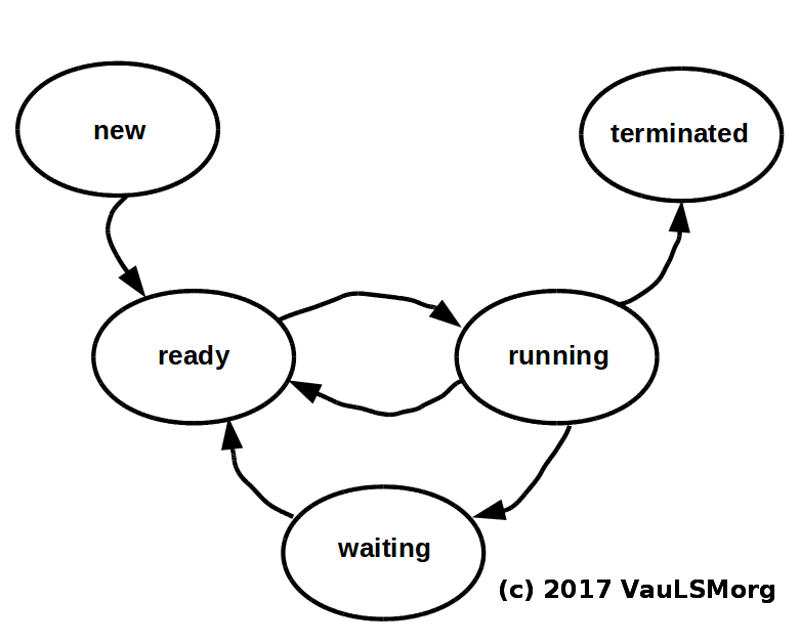
\includegraphics[width=0.55\linewidth]{os06-state}
\caption{A Process State}
\end{figure}
\end{frame}

% XXXXXXXXXXXXXXXXXXXXXXXXXXXXXXXXXXXXXXXXXXXXXXXXXXXXXXXXXXXXXXXXXXXXXXXXXX
\begin{frame}
\frametitle{Process Scheduling}
\begin{itemize}
\item Scheduling Queue
\item Schedulers
\begin{itemize}
\item Long Term (non VM) vs Short Term (CPU)
\item (I/O vs CPU) Bound Processes
\end{itemize}
\item Context Switch
\item I/O Queue Scheduling
\item Android Systems
\begin{itemize}
\item Dalvik VM Performance Problem: Replaced with ART (Android Runtime).
\item Foreground Processes: with an User Interface (UI) for Videos, Images, Sounds, Texts, etc.
\item Background Processes: with a service with no UI and small memory footprint.
\end{itemize}
\end{itemize}
\end{frame}

% XXXXXXXXXXXXXXXXXXXXXXXXXXXXXXXXXXXXXXXXXXXXXXXXXXXXXXXXXXXXXXXXXXXXXXXXXX
\begin{frame}
\frametitle{Inter-Process Communication (IPC)}
\begin{itemize}
\item Independent vs Cooperating Processes.
\begin{itemize}
\item Cooperation: Information Sharing, Computational Speedup, Modularity, Convenience.
\end{itemize}
\item Shared Memory vs Message Passing.
\begin{itemize}
\item Message Passing: Direct vs Indirect Comunication
\end{itemize}
\item Client-Server Systems
\begin{itemize}
\item Sockets
\item RPC: Remote Procedure Calls
\item Pipes
\end{itemize}
\end{itemize}
\end{frame}

% XXXXXXXXXXXXXXXXXXXXXXXXXXXXXXXXXXXXXXXXXXXXXXXXXXXXXXXXXXXXXXXXXXXXXXXXXX
\begin{frame}
\frametitle{Threads}
\begin{itemize}
\item Single vs Multithreaded Process
\begin{itemize}
\item MultiT Benefits: Responsiveness, Resource Sharing, Economy, Scalability
\end{itemize}
\item Multicore Programming
\begin{itemize}
\item Concurrency vs. Parallelism
\end{itemize}
\item Multithreading Models (Kernel vs User Thread)
\begin{itemize}
\item Many to One
\item One to One
\item Many to Many
\item Multilevel Models
\end{itemize}
\item Threading Issues
\begin{itemize}
\item Parallelism on a multi-core system.
\end{itemize}
\item Pthreads
\end{itemize}
\end{frame}

% XXXXXXXXXXXXXXXXXXXXXXXXXXXXXXXXXXXXXXXXXXXXXXXXXXXXXXXXXXXXXXXXXXXXXXXXXX
\section{Makefile}
\begin{frame}[fragile]
\frametitle{Makefile}
\begin{lstlisting}[basicstyle=\ttfamily\tiny]
CC='gcc'
CFLAGS='-std=c99'
 
P00=00-show-pid
...
P15=15-uas171
P16=16-uas172

EXECS= \
	$(P00) \
	$(P01) \
	....
	$(P15) \
	$(P16) \

all:	$(EXECS)

$(P00): $(P00).c
	$(CC) $(P00).c -o $(P00)

$(P01): $(P01).c
	$(CC) $(P01).c -o $(P01)
...

$(P16): $(P16).c
	$(CC) $(P16).c -o $(P16)

clean:
	rm -f $(EXECS)
\end{lstlisting}
\end{frame}

% XXXXXXXXXXXXXXXXXXXXXXXXXXXXXXXXXXXXXXXXXXXXXXXXXXXXXXXXXXXXXXXXXXXXXXXXXX
\section{00-show-pid}
\begin{frame}[fragile]
\frametitle{00-show-pid}
% \begin{lstlisting}[basicstyle=\ttfamily\tiny]         % 108
% \begin{lstlisting}[basicstyle=\ttfamily\footnotesize] %  72
% \begin{lstlisting}[basicstyle=\ttfamily\small]        %  65
% \begin{lstlisting}[basicstyle=\ttfamily\large]        %  54
\begin{lstlisting}[basicstyle=\ttfamily\footnotesize]
/*
 * (c) 2016-2020 Rahmat M. Samik-Ibrahim
 * https://rahmatm.samik-ibrahim.vlsm.org/
 * This is free software.
 * REV07 Tue Mar 24 12:06:10 WIB 2020
 * START Mon Oct 24 09:42:05 WIB 2016
 */

#include <stdio.h>
#include <unistd.h>
#include <sys/types.h>

void main(void) {
   printf("  [[[ This is 00-show-pid: PID[%d] PPID[%d] ]]]\n",
             getpid(), getppid());
}

>>>>> $ ./00-show-pid

  [[[ This is 00-show-pid: PID[5777] PPID[1350] ]]]

\end{lstlisting}
\end{frame}

% XXXXXXXXXXXXXXXXXXXXXXXXXXXXXXXXXXXXXXXXXXXXXXXXXXXXXXXXXXXXXXXXXXXXXXXXXX
\section{01-fork}
\begin{frame}[fragile]
\frametitle{01-fork}
% \begin{lstlisting}[basicstyle=\ttfamily\tiny]         % 108
% \begin{lstlisting}[basicstyle=\ttfamily\footnotesize] %  72
% \begin{lstlisting}[basicstyle=\ttfamily\small]        %  65
% \begin{lstlisting}[basicstyle=\ttfamily\large]        %  54
\begin{lstlisting}[basicstyle=\ttfamily\tiny]
>>>>> $ cat 01-fork.c ; echo "======" ; ./01-fork 
/* (c) 2016-2017 Rahmat M. Samik-Ibrahim
 * https://rahmatm.samik-ibrahim.vlsm.org/
 * This is free software.
 */
#include <stdio.h>
#include <unistd.h>
#include <sys/types.h>
#include <sys/wait.h>

void main(void) {
   char *iAM="PARENT";
  
   printf("PID[%d] PPID[%d] (START:%s)\n", getpid(), getppid(), iAM);
   if (fork() > 0) {
      sleep(1);     /* LOOK THIS ************** */
      printf("PID[%d] PPID[%d] (IFF0:%s)\n", getpid(), getppid(), iAM);
   } else {
      iAM="CHILD";
      printf("PID[%d] PPID[%d] (ELSE:%s)\n", getpid(), getppid(), iAM);
   }
   printf("PID[%d] PPID[%d] (STOP:%s)\n", getpid(), getppid(), iAM);
}
======
PID[5784] PPID[1350] (START:PARENT)
PID[5785] PPID[5784] (ELSE:CHILD)
PID[5785] PPID[5784] (STOP:CHILD)
PID[5784] PPID[1350] (IFF0:PARENT)
PID[5784] PPID[1350] (STOP:PARENT)
>>>>> $ 

\end{lstlisting}
\end{frame}

% XXXXXXXXXXXXXXXXXXXXXXXXXXXXXXXXXXXXXXXXXXXXXXXXXXXXXXXXXXXXXXXXXXXXXXXXXX
\section{02-fork}
\begin{frame}[fragile]
\frametitle{02-fork}
% \begin{lstlisting}[basicstyle=\ttfamily\tiny]         % 108
% \begin{lstlisting}[basicstyle=\ttfamily\footnotesize] %  72
% \begin{lstlisting}[basicstyle=\ttfamily\small]        %  65
% \begin{lstlisting}[basicstyle=\ttfamily\large]        %  54
\begin{lstlisting}[basicstyle=\ttfamily\tiny]
>>>>> $ cat 02-fork.c ; echo "======" ; ./02-fork 
/* (c) 2016-2017 Rahmat M. Samik-Ibrahim
 * https://rahmatm.samik-ibrahim.vlsm.org/
 * This is free software.
 */
#include <stdio.h>
#include <unistd.h>
#include <sys/types.h>
#include <sys/wait.h>

void main(void) {
   char *iAM="PARENT";
  
   printf("PID[%d] PPID[%d] (START:%s)\n", getpid(), getppid(), iAM);
   if (fork() > 0) {
      printf("PID[%d] PPID[%d] (IFF0:%s)\n", getpid(), getppid(), iAM);
   } else {
      iAM="CHILD";
      printf("PID[%d] PPID[%d] (ELSE:%s)\n", getpid(), getppid(), iAM);
      sleep(1);     /* LOOK THIS ************** */
   }
   printf("PID[%d] PPID[%d] (STOP:%s)\n", getpid(), getppid(), iAM);
}
======
PID[5792] PPID[1350] (START:PARENT)
PID[5792] PPID[1350] (IFF0:PARENT)
PID[5792] PPID[1350] (STOP:PARENT)
PID[5793] PPID[5792] (ELSE:CHILD)
>>>>> $ PID[5793] PPID[1] (STOP:CHILD)
>>>>> $
\end{lstlisting}
\end{frame}

% XXXXXXXXXXXXXXXXXXXXXXXXXXXXXXXXXXXXXXXXXXXXXXXXXXXXXXXXXXXXXXXXXXXXXXXXXX
\section{03-fork}
\begin{frame}[fragile]
\frametitle{03-fork}
% \begin{lstlisting}[basicstyle=\ttfamily\tiny]         % 108
% \begin{lstlisting}[basicstyle=\ttfamily\footnotesize] %  72
% \begin{lstlisting}[basicstyle=\ttfamily\small]        %  65
% \begin{lstlisting}[basicstyle=\ttfamily\large]        %  54
\begin{lstlisting}[basicstyle=\ttfamily\tiny]
>>>>> $ cat 03-fork.c ; echo "======" ; ./03-fork 
/* (c) 2016-2017 Rahmat M. Samik-Ibrahim
 * https://rahmatm.samik-ibrahim.vlsm.org/
 * This is free software.
 */
#include <stdio.h>
#include <unistd.h>
#include <sys/types.h>
#include <sys/wait.h>

void main(void) {
   char *iAM="PARENT";
  
   printf("PID[%d] PPID[%d] (START:%s)\n", getpid(), getppid(), iAM);
   if (fork() > 0) {
      wait(NULL);     /* LOOK THIS ************** */
      printf("PID[%d] PPID[%d] (IFF0:%s)\n", getpid(), getppid(), iAM);
   } else {
      iAM="CHILD";
      printf("PID[%d] PPID[%d] (ELSE:%s)\n", getpid(), getppid(), iAM);
   }
   printf("PID[%d] PPID[%d] (STOP:%s)\n", getpid(), getppid(), iAM);
}
======
PID[5799] PPID[1350] (START:PARENT)
PID[5800] PPID[5799] (ELSE:CHILD)
PID[5800] PPID[5799] (STOP:CHILD)
PID[5799] PPID[1350] (IFF0:PARENT)
PID[5799] PPID[1350] (STOP:PARENT)
>>>>> $ 

\end{lstlisting}
\end{frame}

% XXXXXXXXXXXXXXXXXXXXXXXXXXXXXXXXXXXXXXXXXXXXXXXXXXXXXXXXXXXXXXXXXXXXXXXXXX
\section{01-fork vs 02-fork vs 03-fork}
\begin{frame}[fragile]
\frametitle{01-fork vs 02-fork vs 03-fork}
% \begin{lstlisting}[basicstyle=\ttfamily\tiny]         % 108
% \begin{lstlisting}[basicstyle=\ttfamily\footnotesize] %  72
% \begin{lstlisting}[basicstyle=\ttfamily\small]        %  65
% \begin{lstlisting}[basicstyle=\ttfamily\large]        %  54
\begin{lstlisting}[basicstyle=\ttfamily\footnotesize]
>>>>> $ ./01-fork 
PID[5803] PPID[1350] (START:PARENT)
PID[5804] PPID[5803] (ELSE:CHILD)
PID[5804] PPID[5803] (STOP:CHILD)
PID[5803] PPID[1350] (IFF0:PARENT)
PID[5803] PPID[1350] (STOP:PARENT)
>>>>> $ ./02-fork 
PID[5805] PPID[1350] (START:PARENT)
PID[5805] PPID[1350] (IFF0:PARENT)
PID[5805] PPID[1350] (STOP:PARENT)
PID[5806] PPID[5805] (ELSE:CHILD)
>>>>> $ PID[5806] PPID[1] (STOP:CHILD)
>>>>> $ ./03-fork 
PID[5807] PPID[1350] (START:PARENT)
PID[5808] PPID[5807] (ELSE:CHILD)
PID[5808] PPID[5807] (STOP:CHILD)
PID[5807] PPID[1350] (IFF0:PARENT)
PID[5807] PPID[1350] (STOP:PARENT)
>>>>> $ 
\end{lstlisting}
\end{frame}

% XXXXXXXXXXXXXXXXXXXXXXXXXXXXXXXXXXXXXXXXXXXXXXXXXXXXXXXXXXXXXXXXXXXXXXXXXX
\section{04-sleep}
\begin{frame}[fragile]
\frametitle{04-sleep}
% \begin{lstlisting}[basicstyle=\ttfamily\tiny]         % 108
% \begin{lstlisting}[basicstyle=\ttfamily\footnotesize] %  72
% \begin{lstlisting}[basicstyle=\ttfamily\small]        %  65
% \begin{lstlisting}[basicstyle=\ttfamily\large]        %  54
\begin{lstlisting}[basicstyle=\ttfamily\footnotesize]
#include <stdio.h>
#include <unistd.h>
void main(void) {
   int ii;
   printf("Sleeping 3s with fflush(): ");
   fflush(NULL);
   for (ii=0; ii < 3; ii++) {
      sleep(1); printf("x ");
      fflush(NULL);
   }
   printf("\nSleeping with no fflush(): ");
   for (ii=0; ii < 3; ii++) {
      sleep(1); printf("x ");
   }
   printf("\n");
}
Sleeping 3s with fflush(): x x x 
Sleeping with no fflush(): x x x 
\end{lstlisting}
\end{frame}

% XXXXXXXXXXXXXXXXXXXXXXXXXXXXXXXXXXXXXXXXXXXXXXXXXXXXXXXXXXXXXXXXXXXXXXXXXX
\section{05-fork}
\begin{frame}[fragile]
\frametitle{05a-fork}
% \begin{lstlisting}[basicstyle=\ttfamily\tiny]         % 108
% \begin{lstlisting}[basicstyle=\ttfamily\footnotesize] %  72
% \begin{lstlisting}[basicstyle=\ttfamily\small]        %  65
% \begin{lstlisting}[basicstyle=\ttfamily\large]        %  54
\begin{lstlisting}[basicstyle=\ttfamily\tiny]
#include <stdio.h>
#include <unistd.h>
#include <sys/types.h>
#include <sys/wait.h>

void main(void) {
   printf("Start:           PID[%d] PPID[%d]\n", getpid(), getppid());
   fflush(NULL);
   if (fork() == 0) {
      /* START BLOCK
      execlp("./00-fork", "00-fork", NULL);
         END   BLOCK */
      printf("Child:           ");
   } else {
      wait(NULL);
      printf("Parent:          ");
   }
   printf(        "PID[%d] PPID[%d]  <<< <<< <<<\n", getpid(), getppid());
}

no execlp ===================
Start:           PID[6040] PPID[1350]
Child:           PID[6041] PPID[6040]  <<< <<< <<<
Parent:          PID[6040] PPID[1350]  <<< <<< <<<

\end{lstlisting}
\end{frame}

% XXXXXXXXXXXXXXXXXXXXXXXXXXXXXXXXXXXXXXXXXXXXXXXXXXXXXXXXXXXXXXXXXXXXXXXXXX
\begin{frame}[fragile]
\frametitle{05b-fork}
% \begin{lstlisting}[basicstyle=\ttfamily\tiny]         % 108
% \begin{lstlisting}[basicstyle=\ttfamily\footnotesize] %  72
% \begin{lstlisting}[basicstyle=\ttfamily\small]        %  65
% \begin{lstlisting}[basicstyle=\ttfamily\large]        %  54
\begin{lstlisting}[basicstyle=\ttfamily\tiny]
#include <stdio.h>
#include <unistd.h>
#include <sys/types.h>
#include <sys/wait.h>

void main(void) {
   printf("Start:           PID[%d] PPID[%d]\n", getpid(), getppid());
   fflush(NULL);
   if (fork() == 0) {
      /* START BLOCK
         END   BLOCK */
      execlp("./00-fork", "00-fork", NULL);
      printf("Child:           ");
   } else {
      wait(NULL);
      printf("Parent:          ");
   }
   printf(        "PID[%d] PPID[%d]  <<< <<< <<<\n", getpid(), getppid());
}

execlp ======================
Start:           PID[6007] PPID[1350]
  [[[ This is 00-show-pid: PID[6008] PPID[6007] ]]]
Parent:          PID[6007] PPID[1350]  <<< <<< <<<

\end{lstlisting}
\end{frame}

% XXXXXXXXXXXXXXXXXXXXXXXXXXXXXXXXXXXXXXXXXXXXXXXXXXXXXXXXXXXXXXXXXXXXXXXXXX
\section{06-fork}
\begin{frame}[fragile]
\frametitle{06a-fork}
% \begin{lstlisting}[basicstyle=\ttfamily\tiny]         % 108
% \begin{lstlisting}[basicstyle=\ttfamily\footnotesize] %  72
% \begin{lstlisting}[basicstyle=\ttfamily\small]        %  65
% \begin{lstlisting}[basicstyle=\ttfamily\large]        %  54
\begin{lstlisting}[basicstyle=\ttfamily\tiny]
#include <sys/types.h>
#include <sys/wait.h>
#include <stdio.h>
#include <stdlib.h>
#include <unistd.h>
/*************************************************** main ** */
void main(void) {
   pid_t val1, val2, val3;
   val3 = val2 = val1 = 1000;
   printf("PID==%4d ==== ==== ==== ====\n", getpid());
/* ***** ***** ***** ***** START BLOCK *
   fflush(NULL);
   val1 = fork();
   wait(NULL);
   val2 = fork();
   wait(NULL);
   val3 = fork();
   wait(NULL);
   ***** ***** ***** ***** END** BLOCK */
   printf("VAL1=%4d VAL2=%4d VAL3=%4d\n", val1, val2, val3);
}
======
PID==[13965] ==== ======= ==== =======
VAL1=[01000] VAL2=[01000] VAL3=[01000]
\end{lstlisting}
\end{frame}

% XXXXXXXXXXXXXXXXXXXXXXXXXXXXXXXXXXXXXXXXXXXXXXXXXXXXXXXXXXXXXXXXXXXXXXXXXX
\begin{frame}[fragile]
\frametitle{06b-fork}
% \begin{lstlisting}[basicstyle=\ttfamily\tiny]         % 108
% \begin{lstlisting}[basicstyle=\ttfamily\footnotesize] %  72
% \begin{lstlisting}[basicstyle=\ttfamily\small]        %  65
% \begin{lstlisting}[basicstyle=\ttfamily\large]        %  54
\begin{lstlisting}[basicstyle=\ttfamily\tiny]
#include <sys/types.h>
#include <sys/wait.h>
#include <stdio.h>
#include <stdlib.h>
#include <unistd.h>
/*************************************************** main ** */
void main(void) {
   pid_t val1, val2, val3;
   val3 = val2 = val1 = 1000;
   printf("PID==%4d ==== ==== ==== ====\n", getpid());
   fflush(NULL);
   val1 = fork();
   wait(NULL);
/* ***** ***** ***** ***** START BLOCK *
   val2 = fork();
   wait(NULL);
   val3 = fork();
   wait(NULL);
   ***** ***** ***** ***** END** BLOCK */
   printf("VAL1=%4d VAL2=%4d VAL3=%4d\n", val1, val2, val3);
}
======
PID==[13969] ==== ======= ==== =======
VAL1=[00000] VAL2=[01000] VAL3=[01000]
VAL1=[13970] VAL2=[01000] VAL3=[01000]

\end{lstlisting}
\end{frame}

% XXXXXXXXXXXXXXXXXXXXXXXXXXXXXXXXXXXXXXXXXXXXXXXXXXXXXXXXXXXXXXXXXXXXXXXXXX
\begin{frame}[fragile]
\frametitle{06c-fork}
% \begin{lstlisting}[basicstyle=\ttfamily\tiny]         % 108
% \begin{lstlisting}[basicstyle=\ttfamily\footnotesize] %  72
% \begin{lstlisting}[basicstyle=\ttfamily\small]        %  65
% \begin{lstlisting}[basicstyle=\ttfamily\large]        %  54
\begin{lstlisting}[basicstyle=\ttfamily\tiny]
#include <sys/types.h>
#include <sys/wait.h>
#include <stdio.h>
#include <stdlib.h>
#include <unistd.h>
/*************************************************** main ** */
void main(void) {
   pid_t val1, val2, val3;
   val3 = val2 = val1 = 1000;
   printf("PID==%4d ==== ==== ==== ====\n", getpid());
   fflush(NULL);
   val1 = fork();
   wait(NULL);
   val2 = fork();
   wait(NULL);
/* ***** ***** ***** ***** START BLOCK *
   val3 = fork();
   wait(NULL);
   ***** ***** ***** ***** END** BLOCK */
   printf("VAL1=%4d VAL2=%4d VAL3=%4d\n", val1, val2, val3);
}
======
PID==[13971] ==== ======= ==== =======
VAL1=[00000] VAL2=[00000] VAL3=[01000]
VAL1=[00000] VAL2=[13973] VAL3=[01000]
VAL1=[13972] VAL2=[00000] VAL3=[01000]
VAL1=[13972] VAL2=[13974] VAL3=[01000]

\end{lstlisting}
\end{frame}

% XXXXXXXXXXXXXXXXXXXXXXXXXXXXXXXXXXXXXXXXXXXXXXXXXXXXXXXXXXXXXXXXXXXXXXXXXX
\begin{frame}[fragile]
\frametitle{06d-fork}
% \begin{lstlisting}[basicstyle=\ttfamily\tiny]         % 108
% \begin{lstlisting}[basicstyle=\ttfamily\footnotesize] %  72
% \begin{lstlisting}[basicstyle=\ttfamily\small]        %  65
% \begin{lstlisting}[basicstyle=\ttfamily\large]        %  54
\begin{lstlisting}[basicstyle=\ttfamily\tiny]
#include <sys/types.h>
#include <sys/wait.h>
#include <stdio.h>
#include <stdlib.h>
#include <unistd.h>
/*************************************************** main ** */
void main(void) {
   pid_t val1, val2, val3;
   val3 = val2 = val1 = 1000;
   printf("PID==%4d ==== ==== ==== ====\n", getpid());
   fflush(NULL);
   val1 = fork();
   wait(NULL);
   val2 = fork();
   wait(NULL);
   val3 = fork();
   wait(NULL);
/* ***** ***** ***** ***** START BLOCK * ***** ***** ***** ***** END** BLOCK */
   printf("VAL1=%4d VAL2=%4d VAL3=%4d\n", val1, val2, val3);
}
======
PID==[13976] ==== ======= ==== =======
VAL1=[00000] VAL2=[00000] VAL3=[00000]
VAL1=[00000] VAL2=[00000] VAL3=[13979]
VAL1=[00000] VAL2=[13978] VAL3=[00000]
VAL1=[00000] VAL2=[13978] VAL3=[13980]
VAL1=[13977] VAL2=[00000] VAL3=[00000]
VAL1=[13977] VAL2=[00000] VAL3=[13982]
VAL1=[13977] VAL2=[13981] VAL3=[00000]
VAL1=[13977] VAL2=[13981] VAL3=[13983]

\end{lstlisting}
\end{frame}

% XXXXXXXXXXXXXXXXXXXXXXXXXXXXXXXXXXXXXXXXXXXXXXXXXXXXXXXXXXXXXXXXXXXXXXXXXX
\section{07-execlp}
\begin{frame}[fragile]
\frametitle{07-execlp}
% \begin{lstlisting}[basicstyle=\ttfamily\tiny]         % 108
% \begin{lstlisting}[basicstyle=\ttfamily\footnotesize] %  72
% \begin{lstlisting}[basicstyle=\ttfamily\small]        %  65
% \begin{lstlisting}[basicstyle=\ttfamily\large]        %  54
\begin{lstlisting}[basicstyle=\ttfamily\tiny]
>>>>> $ cat 07-execlp.c 
/* (c) 2019-2020 Rahmat M. Samik-Ibrahim
 * https://rahmatm.samik-ibrahim.vlsm.org/
 * This is free software.
 * REV01 Tue Mar 24 16:29:50 WIB 2020
 * START Mon Dec  9 16:28:36 WIB 2019
 */
#include <stdio.h>
#include <sys/types.h>
#include <unistd.h>
void main(int argc, char* argv[]) {
   printf("START %11s PID[%d]\n", argv[0], getpid());
   if(argc == 1) {
      execlp(argv[0], "EXECLP", "WhatEver", NULL);
   } else {
      printf("ELSE  %11s PID[%d]\n", argv[1], getpid());
   }
   printf("END   %11s PID[%d]\n", argv[0], getpid());
}

$ ./07-execlp 
START ./07-execlp PID[14172]
START      EXECLP PID[14172]
ELSE     WhatEver PID[14172]
END        EXECLP PID[14172]
$ ./07-execlp XYZZYPLUGH
START ./07-execlp PID[14174]
ELSE   XYZZYPLUGH PID[14174]
END   ./07-execlp PID[14174]
$ 

\end{lstlisting}
\end{frame}

% XXXXXXXXXXXXXXXXXXXXXXXXXXXXXXXXXXXXXXXXXXXXXXXXXXXXXXXXXXXXXXXXXXXXXXXXXX
\section{08-fork}
\begin{frame}[fragile]
\frametitle{08-fork}
% \begin{lstlisting}[basicstyle=\ttfamily\tiny]         % 108
% \begin{lstlisting}[basicstyle=\ttfamily\footnotesize] %  72
% \begin{lstlisting}[basicstyle=\ttfamily\small]        %  65
% \begin{lstlisting}[basicstyle=\ttfamily\large]        %  54
\begin{lstlisting}[basicstyle=\ttfamily\tiny]
/* (c) 2005-2017 Rahmat M. Samik-Ibrahim https://rahmatm.samik-ibrahim.vlsm.org/ This is free software.
 * REV02 Thu Oct 26 12:27:30 WIB 2017
 * START 2005
 */
#include <sys/types.h>
#include <sys/wait.h>
#include <stdio.h>
#include <stdlib.h>
#include <unistd.h>
void main(void) {
   int ii=0;
   if (fork() == 0) ii++;
   wait(NULL);
   if (fork() == 0) ii++;
   wait(NULL);
   if (fork() == 0) ii++;
   wait(NULL);
   printf ("Result = %d \n",ii);
   exit(0);
}
======
Result = 3 
Result = 2 
Result = 2 
Result = 1 
Result = 2 
Result = 1 
Result = 1 
Result = 0 
>>>>> $ 

\end{lstlisting}
\end{frame}

% XXXXXXXXXXXXXXXXXXXXXXXXXXXXXXXXXXXXXXXXXXXXXXXXXXXXXXXXXXXXXXXXXXXXXXXXXX
\section{09-fork}
\begin{frame}[fragile]
\frametitle{09-fork}
% \begin{lstlisting}[basicstyle=\ttfamily\tiny]         % 108
% \begin{lstlisting}[basicstyle=\ttfamily\footnotesize] %  72
% \begin{lstlisting}[basicstyle=\ttfamily\small]        %  65
% \begin{lstlisting}[basicstyle=\ttfamily\large]        %  54
\begin{lstlisting}[basicstyle=\ttfamily\tiny]
/*
 * (c) 2015-2017 Rahmat M. Samik-Ibrahim https://rahmatm.samik-ibrahim.vlsm.org/
 * REV03 Mon Oct 30 11:04:10 WIB 2017
 * REV00 Mon Oct 24 10:43:00 WIB 2016
 * START 2015
 */
#include <stdio.h>
#include <sys/types.h>
#include <sys/wait.h>
#include <unistd.h>

void main(void) {
   int value;

   value=fork();
   wait(NULL);
   printf("I am PID[%4d] -- The fork() return value is: %4d)\n", getpid(), value);

   value=fork();
   wait(NULL);
   printf("I am PID[%4d] -- The fork() return value is: %4d)\n", getpid(), value);
}
======
I am PID[6225] -- The fork() return value is:    0)
I am PID[6226] -- The fork() return value is:    0)
I am PID[6225] -- The fork() return value is: 6226)
I am PID[6224] -- The fork() return value is: 6225)
I am PID[6227] -- The fork() return value is:    0)
I am PID[6224] -- The fork() return value is: 6227)
>>>>> $ 

\end{lstlisting}
\end{frame}

% XXXXXXXXXXXXXXXXXXXXXXXXXXXXXXXXXXXXXXXXXXXXXXXXXXXXXXXXXXXXXXXXXXXXXXXXXX
\section{10-fork}
\begin{frame}[fragile]
\frametitle{10-fork}
% \begin{lstlisting}[basicstyle=\ttfamily\tiny]         % 108
% \begin{lstlisting}[basicstyle=\ttfamily\footnotesize] %  72
% \begin{lstlisting}[basicstyle=\ttfamily\small]        %  65
% \begin{lstlisting}[basicstyle=\ttfamily\large]        %  54
\begin{lstlisting}[basicstyle=\ttfamily\tiny]
/* (c) 2016-2017 Rahmat M. Samik-Ibrahim https://rahmatm.samik-ibrahim.vlsm.org/ This is free software.
 * REV02 Mon Oct 30 20:25:44 WIB 2017
 */

#include <stdio.h>
#include <sys/types.h>
#include <sys/wait.h>
#include <unistd.h>

void procStatus(int level) {
   printf("L%d: PID[%d] (PPID[%d])\n", level, getpid(), getppid());
   fflush(NULL);
}

int addLevelAndFork(int level) {
   if (fork() == 0) level++;
   wait(NULL);
   return level;
}

void main(void) {
   int level = 0;
   procStatus(level);
   level = addLevelAndFork(level);
   procStatus(level);
}
======
L0: PID[7540] (PPID[1350])
L1: PID[7541] (PPID[7540])
L0: PID[7540] (PPID[1350])

\end{lstlisting}
\end{frame}

% XXXXXXXXXXXXXXXXXXXXXXXXXXXXXXXXXXXXXXXXXXXXXXXXXXXXXXXXXXXXXXXXXXXXXXXXXX
\section{11-fork}
\begin{frame}[fragile]
\frametitle{11-fork}
% \begin{lstlisting}[basicstyle=\ttfamily\tiny]         % 108
% \begin{lstlisting}[basicstyle=\ttfamily\footnotesize] %  72
% \begin{lstlisting}[basicstyle=\ttfamily\small]        %  65
% \begin{lstlisting}[basicstyle=\ttfamily\large]        %  54
\begin{lstlisting}[basicstyle=\ttfamily\tiny]
/* (c) 2016-2017 Rahmat M. Samik-Ibrahim https://rahmatm.samik-ibrahim.vlsm.org/ This is free software.
 * REV02 Mon Oct 30 20:27:24 WIB 2017
 * START Mon Oct 24 09:42:05 WIB 2016
 */

#define  LOOP   3
#include <stdio.h>
#include <sys/types.h>
#include <sys/wait.h>
#include <unistd.h>

void procStatus(int level) {
   printf("L%d: PID[%d] (PPID[%d])\n", level, getpid(), getppid());
   fflush(NULL);
}

int addLevelAndFork(int level) {
   if (fork() == 0) level++;
   wait(NULL);
   return level;
}

void main(void) {
   int ii, level = 0;
   procStatus(level);
   for (ii=0;ii<LOOP;ii++) {
      level = addLevelAndFork(level);
      procStatus(level);
   }
}
 
\end{lstlisting}
\end{frame}

% XXXXXXXXXXXXXXXXXXXXXXXXXXXXXXXXXXXXXXXXXXXXXXXXXXXXXXXXXXXXXXXXXXXXXXXXXX
\begin{frame}[fragile]
\frametitle{11-fork (2)}
% \begin{lstlisting}[basicstyle=\ttfamily\tiny]         % 108
% \begin{lstlisting}[basicstyle=\ttfamily\footnotesize] %  72
% \begin{lstlisting}[basicstyle=\ttfamily\small]        %  65
% \begin{lstlisting}[basicstyle=\ttfamily\large]        %  54
\begin{lstlisting}[basicstyle=\ttfamily\footnotesize]

L0: PID[7548] (PPID[1350])
L1: PID[7549] (PPID[7548])
L2: PID[7550] (PPID[7549])
L3: PID[7551] (PPID[7550])
L2: PID[7550] (PPID[7549])
L1: PID[7549] (PPID[7548])
L2: PID[7552] (PPID[7549])
L1: PID[7549] (PPID[7548])
L0: PID[7548] (PPID[1350])
L1: PID[7553] (PPID[7548])
L2: PID[7554] (PPID[7553])
L1: PID[7553] (PPID[7548])
L0: PID[7548] (PPID[1350])
L1: PID[7555] (PPID[7548])
L0: PID[7548] (PPID[1350])

\end{lstlisting}
\end{frame}

% XXXXXXXXXXXXXXXXXXXXXXXXXXXXXXXXXXXXXXXXXXXXXXXXXXXXXXXXXXXXXXXXXXXXXXXXXX
\section{12-fork}
\begin{frame}[fragile]
\frametitle{12-fork}
% \begin{lstlisting}[basicstyle=\ttfamily\tiny]         % 108
% \begin{lstlisting}[basicstyle=\ttfamily\footnotesize] %  72
% \begin{lstlisting}[basicstyle=\ttfamily\small]        %  65
% \begin{lstlisting}[basicstyle=\ttfamily\large]        %  54
\begin{lstlisting}[basicstyle=\ttfamily\tiny]
#include <stdio.h>
#include <unistd.h>
#include <sys/types.h>
#include <sys/wait.h>
void waitAndPrintPID(void) {
   wait(NULL);
   printf("PID: %d\n", getpid());
   fflush(NULL);
}
void main(int argc, char *argv[]) {
   int rc, status;
   waitAndPrintPID();
   rc = fork();
   waitAndPrintPID();
   if (rc == 0) {
      fork();
      waitAndPrintPID();
      execlp("./00-fork", "00-fork", NULL);
   }
   waitAndPrintPID();
}
======
PID: 7614
PID: 7615
PID: 7616
  [[[ This is 00-fork: PID[7616] PPID[7615] ]]]
PID: 7615
  [[[ This is 00-fork: PID[7615] PPID[7614] ]]]
PID: 7614
PID: 7614
>>>>> $ 

\end{lstlisting}
\end{frame}

% XXXXXXXXXXXXXXXXXXXXXXXXXXXXXXXXXXXXXXXXXXXXXXXXXXXXXXXXXXXXXXXXXXXXXXXXXX
\section{13-uas161}
\begin{frame}[fragile]
\frametitle{13-uas161}
% \begin{lstlisting}[basicstyle=\ttfamily\tiny]         % 108
% \begin{lstlisting}[basicstyle=\ttfamily\footnotesize] %  72
% \begin{lstlisting}[basicstyle=\ttfamily\small]        %  65
% \begin{lstlisting}[basicstyle=\ttfamily\large]        %  54
\begin{lstlisting}[basicstyle=\ttfamily\tiny]
/*
 * Copyright (C) 2015-2020 Rahmat M. Samik-Ibrahim http://rahmatm.samik-ibrahim.vlsm.org/ This program is free script/software.
 * REV10 Tue Mar 24 16:38:29 WIB 2020
 * START Xxx Xxx XX XX:XX:XX XXX XXXX
 */

#include <stdio.h>
#include <unistd.h>
#include <sys/types.h>
#include <sys/wait.h>

void main(void) {
   pid_t  pid1, pid2, pid3;

   pid1 = pid2 = pid3 = getpid();
   printf(" 2016   2015   Lainnya\n=====================\n");
   printf("[%5.5d][%5.5d][%5.5d]\n", pid1, pid2, pid3);
   fork(); 
   pid1 = getpid();
   wait(NULL);
   pid2 = getpid();
   if(!fork()) {
     pid2 = getpid();
     fork();
   }
   pid3 = getpid();
   wait(NULL);
   printf("[%5.5d][%5.5d][%5.5d]\n", pid1, pid2, pid3);
}

/*
# INFO: UTS 2016-1 (midterm)
 */

\end{lstlisting}
\end{frame}

% XXXXXXXXXXXXXXXXXXXXXXXXXXXXXXXXXXXXXXXXXXXXXXXXXXXXXXXXXXXXXXXXXXXXXXXXXX
\begin{frame}[fragile]
\frametitle{13-uas161}
% \begin{lstlisting}[basicstyle=\ttfamily\tiny]         % 108
% \begin{lstlisting}[basicstyle=\ttfamily\footnotesize] %  72
% \begin{lstlisting}[basicstyle=\ttfamily\small]        %  65
\begin{lstlisting}[basicstyle=\ttfamily\large]        %  54

/*
# INFO: UTS 2016-1 (midterm)
 */

$ ./13-uas161 
 2016   2015   Lainnya
=====================
[14492][14492][14492]
[14493][14494][14495]
[14493][14494][14494]
[14493][14493][14493]
[14492][14496][14497]
[14492][14496][14496]
[14492][14492][14492]

\end{lstlisting}
\end{frame}

% XXXXXXXXXXXXXXXXXXXXXXXXXXXXXXXXXXXXXXXXXXXXXXXXXXXXXXXXXXXXXXXXXXXXXXXXXX
\section{14-uas162}
\begin{frame}[fragile]
\frametitle{14-uas162}
\begin{lstlisting}[basicstyle=\ttfamily\tiny]         % 108
% \begin{lstlisting}[basicstyle=\ttfamily\footnotesize] %  72
% \begin{lstlisting}[basicstyle=\ttfamily\small]        %  65
% \begin{lstlisting}[basicstyle=\ttfamily\large]        %  54

/* Copyright (C) 2016-2020 Rahmat M. Samik-Ibrahim http://rahmatm.samik-ibrahim.vlsm.org/
 * This program is free script/software.
 * REV08 Tue Mar 24 16:40:28 WIB 2020
 * START Sun Dec 04 00:00:00 WIB 2016
 * wait()     =  suspends until its child terminates. 
 * fflush()   =  flushes the user-space buffers.
 * getppid()  =  get parent PID
 * ASSUME pid >= 1000 && pid > ppid **
 */

#include <stdio.h>
#include <sys/types.h>
#include <unistd.h>
#include <sys/wait.h>
#define  NN 2

void main(void) {
   int ii, rPID, rPPID, id1000=getpid();
   for (ii=1; ii<=NN; ii++) {
      fork();
      wait(NULL);
      rPID = getpid()-id1000+1000; /* "relative" */
      rPPID=getppid()-id1000+1000; /* "relative" */
      if (rPPID < 1000 || rPPID > rPID) rPPID=999;
      printf("Loop [%d] - rPID[%d] - rPPID[%4d]\n", ii, rPID, rPPID);
      fflush(NULL);
   }
}

\end{lstlisting}
\end{frame}

% XXXXXXXXXXXXXXXXXXXXXXXXXXXXXXXXXXXXXXXXXXXXXXXXXXXXXXXXXXXXXXXXXXXXXXXXXX
\begin{frame}[fragile]
\frametitle{14-uas162}
% \begin{lstlisting}[basicstyle=\ttfamily\tiny]         % 108
% \begin{lstlisting}[basicstyle=\ttfamily\footnotesize] %  72
% \begin{lstlisting}[basicstyle=\ttfamily\small]        %  65
\begin{lstlisting}[basicstyle=\ttfamily\large]        %  54

/*
# INFO: UTS 2016-2 (midterm)
 */

$ ./14-uas162 
Loop [1] - rPID[1001] - rPPID[1000]
Loop [2] - rPID[1002] - rPPID[1001]
Loop [2] - rPID[1001] - rPPID[1000]
Loop [1] - rPID[1000] - rPPID[ 999]
Loop [2] - rPID[1003] - rPPID[1000]
Loop [2] - rPID[1000] - rPPID[ 999]

\end{lstlisting}
\end{frame}

% XXXXXXXXXXXXXXXXXXXXXXXXXXXXXXXXXXXXXXXXXXXXXXXXXXXXXXXXXXXXXXXXXXXXXXXXXX
\section{15-uas171}
\begin{frame}[fragile]
\frametitle{15-uas171}
\begin{lstlisting}[basicstyle=\ttfamily\tiny]         % 108
% \begin{lstlisting}[basicstyle=\ttfamily\footnotesize] %  72
% \begin{lstlisting}[basicstyle=\ttfamily\small]        %  65
% \begin{lstlisting}[basicstyle=\ttfamily\large]        %  54

/* Copyright (C) 2005-2020 Rahmat M. Samik-Ibrahim http://rahmatm.samik-ibrahim.vlsm.org/ This program is free script/software. 
 * REV00 Wed May  3 17:07:09 WIB 2017
 * START 2005
 * fflush(NULL): flushes all open output streams
 * fork():       creates  a new process by cloning
 * getpid():     get PID (Process ID)
 * wait(NULL):   wait until the child is terminated
 */

#include <stdio.h>
#include <unistd.h>
#include <sys/types.h>
#include <sys/wait.h>
#include <stdlib.h>

void main(void) {
   int firstPID = (int) getpid();
   int   RelPID;

   fork();
   wait(NULL);
   fork();
   wait(NULL);
   fork();
   wait(NULL);

   RelPID=(int)getpid()-firstPID+1000;
   printf("RelPID: %d\n", RelPID);
   fflush(NULL);
}

\end{lstlisting}
\end{frame}

% XXXXXXXXXXXXXXXXXXXXXXXXXXXXXXXXXXXXXXXXXXXXXXXXXXXXXXXXXXXXXXXXXXXXXXXXXX
\begin{frame}[fragile]
\frametitle{15-uas171}
% \begin{lstlisting}[basicstyle=\ttfamily\tiny]         % 108
% \begin{lstlisting}[basicstyle=\ttfamily\footnotesize] %  72
% \begin{lstlisting}[basicstyle=\ttfamily\small]        %  65
\begin{lstlisting}[basicstyle=\ttfamily\large]        %  54

/*
# INFO: UTS 2017-1 (midterm)
 */

$ ./15-uas171 
RelPID: 1003
RelPID: 1002
RelPID: 1004
RelPID: 1001
RelPID: 1006
RelPID: 1005
RelPID: 1007
RelPID: 1000
$ 


\end{lstlisting}
\end{frame}

% XXXXXXXXXXXXXXXXXXXXXXXXXXXXXXXXXXXXXXXXXXXXXXXXXXXXXXXXXXXXXXXXXXXXXXXXXX
\section{16-uas172}
\begin{frame}[fragile]
\frametitle{16-uas172}
\begin{lstlisting}[basicstyle=\ttfamily\tiny]         % 108
% \begin{lstlisting}[basicstyle=\ttfamily\footnotesize] %  72
% \begin{lstlisting}[basicstyle=\ttfamily\small]        %  65
% \begin{lstlisting}[basicstyle=\ttfamily\large]        %  54

/*
 * (c) 2017-2020 Rahmat M. Samik-Ibrahim
 * http://rahmatm.samik-ibrahim.vlsm.org/
 * This is free software.
 * REV03 Tue Mar 24 16:42:16 WIB 2020
 * REV02 Mon Dec 11 17:46:01 WIB 2017
 * START Sun Dec  3 18:00:08 WIB 2017
 */

#include <stdio.h>
#include <unistd.h>
#include <sys/types.h>
#include <sys/wait.h>

#define LOOP   3
#define OFFSET 1000

void main(void) {
   int basePID = getpid() - OFFSET;

   for (int ii=0; ii < LOOP; ii++) {
      if(!fork()) {
         printf("PID[%d]-PPID[%d]\n", 
                 getpid()  - basePID, 
                 getppid() - basePID);
         fflush(NULL);
      }
      wait(NULL);
   }
}

\end{lstlisting}
\end{frame}

% XXXXXXXXXXXXXXXXXXXXXXXXXXXXXXXXXXXXXXXXXXXXXXXXXXXXXXXXXXXXXXXXXXXXXXXXXX
\begin{frame}[fragile]
\frametitle{16-uas172}
% \begin{lstlisting}[basicstyle=\ttfamily\tiny]         % 108
% \begin{lstlisting}[basicstyle=\ttfamily\footnotesize] %  72
% \begin{lstlisting}[basicstyle=\ttfamily\small]        %  65
\begin{lstlisting}[basicstyle=\ttfamily\large]        %  54

/*
# INFO: UTS 2017-2 (midterm)
 */

$ ./16-uas172 
PID[1001]-PPID[1000]
PID[1002]-PPID[1001]
PID[1003]-PPID[1002]
PID[1004]-PPID[1001]
PID[1005]-PPID[1000]
PID[1006]-PPID[1005]
PID[1007]-PPID[1000]
$ 

\end{lstlisting}
\end{frame}

% XXXXXXXXXXXXXXXXXXXXXXXXXXXXXXXXXXXXXXXXXXXXXXXXXXXXXXXXXXXXXXXXXXXXXXXXXX
\section{Assignment Week06}
\begin{frame}[fragile]
\frametitle{mylib.h (1)}
% \begin{lstlisting}[basicstyle=\ttfamily\tiny]         % 108
% \begin{lstlisting}[basicstyle=\ttfamily\footnotesize] %  72
% \begin{lstlisting}[basicstyle=\ttfamily\small]        %  65
% \begin{lstlisting}[basicstyle=\ttfamily\large]        %  54
\begin{lstlisting}[basicstyle=\ttfamily\tiny]         % 108

/*
 * Copyright (C) 2021-2021 Rahmat M. Samik-Ibrahim
 * http://rahmatm.samik-ibrahim.vlsm.org/
 * This program is free script/software. This program is distributed in the
 * hope that it will be useful, but WITHOUT ANY WARRANTY; without even the
 * implied warranty of MERCHANTABILITY or FITNESS FOR A PARTICULAR PURPOSE.
 * REV08: Sun 04 Apr 07:28:09 WIB 2021
 * REV07: Sun 04 Apr 00:11:43 WIB 2021
 * REV06: Sat 03 Apr 11:00:46 WIB 2021
 * REV05: Tue 30 Mar 14:55:36 WIB 2021
 * REV04: Tue 30 Mar 10:35:13 WIB 2021
 * START: Mon 22 Mar 16:14:36 WIB 2021
 *
# INFO: mylib.h
 */

#define TOKEN          "OS212W06"
#define WEEKFILE       "WEEK06-MEMORY-SHARE.bin"
#define FORKS          4

#define BUFFERSIZE     256
#define SSIZE          4
#define STAMPSIZE      11
#define CHMOD          0666
#define CMDSHA1 "echo %s | sha1sum | cut -c1-4 | tr '[:lower:]' '[:upper:]' "
#define MYFLAGS        O_CREAT|O_RDWR
#define MYPROTECTION   PROT_READ|PROT_WRITE
#define MYVISIBILITY   MAP_SHARED

\end{lstlisting}
\end{frame}

% 10 XXXXXXXXXXXXXXXXXXXXXXXXXXXXXXXXXXXXXXXXXXXXXXXXXXXXXXXXXXXXXXXXXXXXXXXX
\begin{frame}[fragile]
\frametitle{mylib.h (2)}
% \begin{lstlisting}[basicstyle=\ttfamily\tiny]         % 108
% \begin{lstlisting}[basicstyle=\ttfamily\footnotesize] %  72
% \begin{lstlisting}[basicstyle=\ttfamily\small]        %  65
% \begin{lstlisting}[basicstyle=\ttfamily\large]        %  54
% \end{lstlisting}
% \end{frame}
\begin{lstlisting}[basicstyle=\ttfamily\tiny]         % 108

#include <fcntl.h>
#include <stdio.h>
#include <stdlib.h>
#include <string.h>
#include <sys/mman.h>
#include <sys/stat.h>
#include <sys/types.h>
#include <sys/wait.h>
#include <time.h>
#include <unistd.h>

typedef           char  Chr;
typedef           char* ChrPtr;
typedef  unsigned char  uChr;
typedef  unsigned char* uChrPtr;
typedef  struct {
    Chr counter;
    Chr blank;
    Chr stamp[FORKS][BUFFERSIZE];
    Chr end;
    Chr zero;
} memStruct;
typedef memStruct* memStructPtr;

void            chktoken         (uChrPtr result, uChrPtr token);
memStructPtr createShareMemory(memStructPtr mymap, int memorySize, ChrPtr memoryName);
void            getTimeStamp     (uChrPtr timeStamp);
void            mySHA1           (uChrPtr output, uChrPtr input, int length);
void            pickToken        (uChrPtr result, uChrPtr token);
void            verifyToken      (uChrPtr result, uChrPtr token, uChrPtr input);

\end{lstlisting}
\end{frame}

% 10 XXXXXXXXXXXXXXXXXXXXXXXXXXXXXXXXXXXXXXXXXXXXXXXXXXXXXXXXXXXXXXXXXXXXXXXX
\begin{frame}[fragile]
\frametitle{mylib.c (1)}
% \begin{lstlisting}[basicstyle=\ttfamily\tiny]         % 108
% \begin{lstlisting}[basicstyle=\ttfamily\footnotesize] %  72
% \begin{lstlisting}[basicstyle=\ttfamily\small]        %  65
% \begin{lstlisting}[basicstyle=\ttfamily\large]        %  54
\begin{lstlisting}[basicstyle=\ttfamily\tiny]         % 108

/*
 * Copyright (C) 2021-2021 Rahmat M. Samik-Ibrahim
 * http://rahmatm.samik-ibrahim.vlsm.org/
 * This program is free script/software. This program is distributed in the 
 * hope that it will be useful, but WITHOUT ANY WARRANTY; without even the 
 * implied warranty of MERCHANTABILITY or FITNESS FOR A PARTICULAR PURPOSE.
 * REV08: Sun 04 Apr 07:25:24 WIB 2021
 * REV07: Sun 04 Apr 00:11:43 WIB 2021
 * REV04: Tue 30 Mar 10:35:13 WIB 2021
 * START: Mon 22 Mar 16:14:36 WIB 2021
 *
# INFO: mylib.c
 */

#include "mylib.h"

void mySHA1(uChrPtr output, uChrPtr input, int length) {
    Chr     cmd[BUFFERSIZE];
    sprintf(cmd, CMDSHA1, input);
    FILE* filePtr = popen(cmd, "r");
    fgets(output, length+1, filePtr);
    output[length]=0;
    pclose(filePtr);
}

void getTimeStamp(uChrPtr timeStamp) {
    time_t tt    =  time(NULL);
    struct tm tm = *localtime(&tt);
    sprintf(timeStamp, "%2.2d%2.2d", tm.tm_min, tm.tm_sec);
}

\end{lstlisting}
\end{frame}

% 10 XXXXXXXXXXXXXXXXXXXXXXXXXXXXXXXXXXXXXXXXXXXXXXXXXXXXXXXXXXXXXXXXXXXXXXXX
\begin{frame}[fragile]
\frametitle{mylib.c (2)}
% \begin{lstlisting}[basicstyle=\ttfamily\tiny]         % 108
% \begin{lstlisting}[basicstyle=\ttfamily\footnotesize] %  72
% \begin{lstlisting}[basicstyle=\ttfamily\small]        %  65
% \begin{lstlisting}[basicstyle=\ttfamily\large]        %  54
\begin{lstlisting}[basicstyle=\ttfamily\tiny]         % 108

void chktoken (uChrPtr result, uChrPtr token) {
    uChr timeStamp[] = "MMSS";
    getTimeStamp(timeStamp);
    uChr input [BUFFERSIZE];
    strcpy(input,timeStamp);
    uChrPtr user=getenv("USER");
    strcat(input,user);
    strcat(input,token);
    uChr   output [BUFFERSIZE];
    mySHA1(output, input, SSIZE);
    sprintf(result, "%s %s-%s", user, timeStamp, output);
}

void verifyToken(uChrPtr result, uChrPtr token, uChrPtr input) {
    uChr    tmpStr1[BUFFERSIZE];
    uChr    tmpStr2[BUFFERSIZE];
    strcpy(tmpStr1,input);
    uChrPtr user=strtok(tmpStr1," ");
    uChrPtr timeStamp=strtok(NULL,"-");
    strcpy(tmpStr2,timeStamp);
    strcat(tmpStr2,user);
    strcat(tmpStr2,token);
    uChr   output [BUFFERSIZE];
    mySHA1(output, tmpStr2, SSIZE);
    uChrPtr tmpStr3=strtok(NULL,"-");
    if (strcmp(output, tmpStr3) == 0 ) sprintf(result, "Verified");
    else sprintf(result, "Error");
}

\end{lstlisting}
\end{frame}

% 10 XXXXXXXXXXXXXXXXXXXXXXXXXXXXXXXXXXXXXXXXXXXXXXXXXXXXXXXXXXXXXXXXXXXXXXXX
\begin{frame}[fragile]
\frametitle{mylib.c (3)}
% \begin{lstlisting}[basicstyle=\ttfamily\footnotesize] %  72
% \begin{lstlisting}[basicstyle=\ttfamily\small]        %  65
% \begin{lstlisting}[basicstyle=\ttfamily\large]        %  54
\begin{lstlisting}[basicstyle=\ttfamily\tiny]         % 108

void pickToken (uChrPtr result, uChrPtr token) {
    uChr   tmpStr1[BUFFERSIZE];
    strcpy(tmpStr1,token);
    strtok(tmpStr1," ");
    strcpy(result, strtok(NULL," "));
}

memStructPtr createShareMemory(memStructPtr mymap, int memorySize, ChrPtr memoryName) {
    int      fd    = open(memoryName, MYFLAGS, CHMOD);
    fchmod   (fd, CHMOD);
    ftruncate(fd, memorySize);
    mymap = mmap(NULL, memorySize, MYPROTECTION, MYVISIBILITY, fd, 0);
    close(fd);
    return mymap;
}

\end{lstlisting}
\end{frame}

% 10 XXXXXXXXXXXXXXXXXXXXXXXXXXXXXXXXXXXXXXXXXXXXXXXXXXXXXXXXXXXXXXXXXXXXXXXX
\begin{frame}[fragile]
\frametitle{chktoken.c (1)}
% \begin{lstlisting}[basicstyle=\ttfamily\footnotesize] %  72
% \begin{lstlisting}[basicstyle=\ttfamily\small]        %  65
% \begin{lstlisting}[basicstyle=\ttfamily\large]        %  54
\begin{lstlisting}[basicstyle=\ttfamily\tiny]         % 108

/*
 * Copyright (C) 2021-2021 Rahmat M. Samik-Ibrahim
 * http://rahmatm.samik-ibrahim.vlsm.org/
 * This program is free script/software. This program is distributed in the 
 * hope that it will be useful, but WITHOUT ANY WARRANTY; without even the 
 * implied warranty of MERCHANTABILITY or FITNESS FOR A PARTICULAR PURPOSE.
# INFO: chktoken TOKEN
 * REV02 Sun 04 Apr 2021 08:05:57 WIB
 * REV01 Sun 04 Apr 2021 00:11:27 WIB
 * START Sat 03 Apr 2021 15:10:28 WIB
 */

#include "mylib.h"

int main(int argc, ChrPtr argv[]) {
    if (argc < 2) return -1;
    uChr     result1[BUFFERSIZE];
    chktoken (result1, argv[1]);
    printf("%s\n", result1);
}

\end{lstlisting}
\end{frame}

% 10 XXXXXXXXXXXXXXXXXXXXXXXXXXXXXXXXXXXXXXXXXXXXXXXXXXXXXXXXXXXXXXXXXXXXXXXX
\begin{frame}[fragile]
\frametitle{verifyToken.c (1)}
% \begin{lstlisting}[basicstyle=\ttfamily\footnotesize] %  72
% \begin{lstlisting}[basicstyle=\ttfamily\small]        %  65
% \begin{lstlisting}[basicstyle=\ttfamily\large]        %  54
\begin{lstlisting}[basicstyle=\ttfamily\tiny]         % 108

/*
 * Copyright (C) 2021-2021 Rahmat M. Samik-Ibrahim
 * http://rahmatm.samik-ibrahim.vlsm.org/
 * This program is free script/software. This program is distributed in the 
 * hope that it will be useful, but WITHOUT ANY WARRANTY; without even the 
 * implied warranty of MERCHANTABILITY or FITNESS FOR A PARTICULAR PURPOSE.
# INFO: TOP (Table of Processes)
 * REV02 Sun 04 Apr 2021 07:24:22 WIB
 * REV01 Sun 04 Apr 2021 00:11:27 WIB
 * START Sat 03 Apr 2021 15:10:28 WIB
 */

#include "mylib.h"

int main(int argc, ChrPtr argv[]) {
    if (argc < 4) return -1;
    uChr     result1[BUFFERSIZE];
    uChr     result2[BUFFERSIZE];
    strcpy(result1,argv[2]);
    strcat(result1," ");
    strcat(result1,argv[3]);
    verifyToken(result2, argv[1], result1);
    printf("%s\n", result2);
}

\end{lstlisting}
\end{frame}

% 10 XXXXXXXXXXXXXXXXXXXXXXXXXXXXXXXXXXXXXXXXXXXXXXXXXXXXXXXXXXXXXXXXXXXXXXXX
\begin{frame}[fragile]
\frametitle{myfork.c (1)}
% \begin{lstlisting}[basicstyle=\ttfamily\footnotesize] %  72
% \begin{lstlisting}[basicstyle=\ttfamily\small]        %  65
% \begin{lstlisting}[basicstyle=\ttfamily\large]        %  54
\begin{lstlisting}[basicstyle=\ttfamily\tiny]         % 108

/*
 * Copyright (C) 2021-2021 Rahmat M. Samik-Ibrahim
 * http://rahmatm.samik-ibrahim.vlsm.org/
 * This program is free script/software. This program is distributed in the 
 * hope that it will be useful, but WITHOUT ANY WARRANTY; without even the 
 * implied warranty of MERCHANTABILITY or FITNESS FOR A PARTICULAR PURPOSE.
# INFO: myfork00
 * START Sun 04 Apr 2021 11:00:01 AM WIB
 */

#include "mylib.h"

int main(void) {
    memStructPtr  mymap = createShareMemory(mymap, sizeof(memStruct), WEEKFILE);
    mymap->counter='1';
    int counter=mymap->counter-'1';
    mymap->blank=' ';
    mymap->end='\n';
    mymap->zero=0;
    uChr      result1[BUFFERSIZE];
    chktoken (result1, TOKEN);

\end{lstlisting}
\end{frame}

% 10 XXXXXXXXXXXXXXXXXXXXXXXXXXXXXXXXXXXXXXXXXXXXXXXXXXXXXXXXXXXXXXXXXXXXXXXX
\begin{frame}[fragile]
\frametitle{myfork.c (2)}
% \begin{lstlisting}[basicstyle=\ttfamily\footnotesize] %  72
% \begin{lstlisting}[basicstyle=\ttfamily\small]        %  65
% \begin{lstlisting}[basicstyle=\ttfamily\large]        %  54
\begin{lstlisting}[basicstyle=\ttfamily\tiny]         % 108

    if (fork() == 0) {
        sleep(1);
        mymap->counter++;
        counter=mymap->counter-'1';
        chktoken (result1, TOKEN);
        if (fork() == 0) {
            sleep(1);
            mymap->counter++;
            counter=mymap->counter-'1';
            chktoken (result1, TOKEN);
            if (fork() == 0) {
                sleep(1);
                mymap->counter++;
                counter=mymap->counter-'1';
                chktoken (result1, TOKEN);
            }
            wait(NULL);
        }
        wait(NULL);
    }
    wait(NULL);
    strcpy(mymap->stamp[counter], result1);
    strcat(mymap->stamp[counter], " ");
    printf("PID[%d][%s]-[%d]\n", getpid(), result1, counter);
    wait(NULL);
}

\end{lstlisting}
\end{frame}

% 10 XXXXXXXXXXXXXXXXXXXXXXXXXXXXXXXXXXXXXXXXXXXXXXXXXXXXXXXXXXXXXXXXXXXXXXXX
\begin{frame}[fragile]
\frametitle{mytest.c (1)}
% \begin{lstlisting}[basicstyle=\ttfamily\footnotesize] %  72
% \begin{lstlisting}[basicstyle=\ttfamily\small]        %  65
% \begin{lstlisting}[basicstyle=\ttfamily\large]        %  54
\begin{lstlisting}[basicstyle=\ttfamily\tiny]         % 108

/*
 * Copyright (C) 2021-2021 Rahmat M. Samik-Ibrahim
 * http://rahmatm.samik-ibrahim.vlsm.org/
 * This program is free script/software. This program is distributed in the 
 * hope that it will be useful, but WITHOUT ANY WARRANTY; without even the 
 * implied warranty of MERCHANTABILITY or FITNESS FOR A PARTICULAR PURPOSE.
# INFO: TOP (Table of Processes)
 * REV01 Sun 04 Apr 2021 00:11:59 WIB
 * START Sat 03 Apr 2021 15:10:28 WIB
 */

#include "mylib.h"

int main(void) {
    uChr     result1[BUFFERSIZE];
    chktoken (result1, TOKEN);
    printf("%s\n", result1);
    uChr     result2[BUFFERSIZE];
    verifyToken (result2, TOKEN, result1);
    printf("%s: %s\n", TOKEN, result2);
    verifyToken (result2, "DODOLGRT", "rms46 0605-0687");
    printf("%s: %s\n", "DODOLGRT", result2);
    verifyToken (result2, "DODOLGRT", "rms46 1820-2A46");
    printf("%s: %s\n", "DODOLGRT", result2);
    sleep (1);
    chktoken (result1, TOKEN);
    printf("%s\n", result1);
    pickToken(result2, result1);
    printf("%s\n", result2);
}

\end{lstlisting}
\end{frame}

% 10 XXXXXXXXXXXXXXXXXXXXXXXXXXXXXXXXXXXXXXXXXXXXXXXXXXXXXXXXXXXXXXXXXXXXXXXX
\begin{frame}[fragile]
\frametitle{mytest.sh (1)}
% \begin{lstlisting}[basicstyle=\ttfamily\footnotesize] %  72
% \begin{lstlisting}[basicstyle=\ttfamily\small]        %  65
% \begin{lstlisting}[basicstyle=\ttfamily\large]        %  54
\begin{lstlisting}[basicstyle=\ttfamily\tiny]         % 108

#!/bin/bash
# REV01 Mon  5 Apr 17:08:58 WIB 2021
# START Sun  4 Apr 17:22:46 WIB 2021
# Copyright (C) 2021-2021 Rahmat M. Samik-Ibrahim http://rahmatm.samik-ibrahim.vlsm.org/
# This program is free script/software. This program is distributed in the 
# hope that it will be useful, but WITHOUT ANY WARRANTY; without even the 
# implied warranty of MERCHANTABILITY or FITNESS FOR A PARTICULAR PURPOSE.
# INFO: myfork00

CLEANFILE="WEEK06-MEMORY-SHARE.txt"
WEEKFILE="WEEK06-MEMORY-SHARE.bin"

TOKEN="OS212W06"

[ -f $CLEANFILE ] || { echo "No $CLEANFILE"; exit; }

sleep 1
echo "ZCZC $(date)"
echo -n "ZCZC $(./chktoken $TOKEN): "
echo "$(./verifyToken $TOKEN $(./chktoken $TOKEN))"
echo "ZCZC BINSIZE $(wc -c < $WEEKFILE)"
echo "ZCZC TXTSIZE $(wc -c < $CLEANFILE)"
FIRST=""
for II in $(cat $CLEANFILE) ; do
    [ ! -z "${II##*[!0-9]*}" ] && continue
    [ -z "$FIRST" ] && { FIRST=$II ; continue; }
    echo -n "ZCZC $FIRST $II: "
    echo "$(./verifyToken $TOKEN $FIRST $II)"
    FIRST=""
done

\end{lstlisting}
\end{frame}

% 10 XXXXXXXXXXXXXXXXXXXXXXXXXXXXXXXXXXXXXXXXXXXXXXXXXXXXXXXXXXXXXXXXXXXXXXXX
\begin{frame}[fragile]
\frametitle{Makefile (1)}
% \begin{lstlisting}[basicstyle=\ttfamily\footnotesize] %  72
% \begin{lstlisting}[basicstyle=\ttfamily\small]        %  65
% \begin{lstlisting}[basicstyle=\ttfamily\large]        %  54
\begin{lstlisting}[basicstyle=\ttfamily\tiny]         % 108

# REV03 Mon 05 Apr 17:55:47 WIB 2021
# REV02 Sun 04 Apr 07:22:23 WIB 2021
# REV01 Sat 03 Apr 10:51:58 WIB 2021
# START Tue 13 Sep 11:44:18 WIB 2016

# INFO: With this "Makefile", just run:
# INFO:                     make

CC            = gcc
CPP           = cpp
CFLAGS        = -std=gnu18
LDFLAGS       = 
CPPFLAGS      =
DEPFLAGS      = -MM -MT $(@:.d=.o) 
OUTPUT_OPTION = -o $@
COMPILE       = $(CC) $(DEPFLAGS) $(CFLAGS) $(CPPFLAGS) -c
SRCS          = $(wildcard *.c)
OBJ           = $(SRCS:.c=.o)
DEP           = $(OBJ:.o=.d)
PROGS         = $(SRCS:.c=  )

P01=mytest
P02=chktoken
P03=verifyToken
P04=myfork

L99=mylib
WEEKFILE=WEEK06-MEMORY-SHARE.bin
CLEANFILE=WEEK06-MEMORY-SHARE.txt

\end{lstlisting}
\end{frame}

% 10 XXXXXXXXXXXXXXXXXXXXXXXXXXXXXXXXXXXXXXXXXXXXXXXXXXXXXXXXXXXXXXXXXXXXXXXX
\begin{frame}[fragile]
\frametitle{Makefile (2)}
% \begin{lstlisting}[basicstyle=\ttfamily\footnotesize] %  72
% \begin{lstlisting}[basicstyle=\ttfamily\small]        %  65
% \begin{lstlisting}[basicstyle=\ttfamily\large]        %  54
\begin{lstlisting}[basicstyle=\ttfamily\tiny]         % 108

EXECS= \
   $(P01) \
   $(P02) \
   $(P03) \
   $(P04) \


all:  $(EXECS)

test: $(EXECS)
	./$(P04) 
	cat $(WEEKFILE) | wc -c > $(CLEANFILE)
	cat $(WEEKFILE) | tr -dc '[:alnum:]\n -_' >> $(CLEANFILE)
	bash mytest.sh

$(EXECS): %: %.c $(DEPS) $(L99).c
	$(CC) $(CFLAGS)  $(L99).c $< -o $@ $(LDFLAGS)

clean:
	rm -f $(EXECS)
	rm -f *.map 
	rm -f $(WEEKFILE) $(CLEANFILE)

.phony: clean all test

\end{lstlisting}
\begin{table}
\end{table}
\end{frame}

% XXXXXXXXXXXXXXXXXXXXXXXXXXXXXXXXXXXXXXXXXXXXXXXXXXXXXXXXXXXXXXXXXXXXXXXXXX
\end{document}

